\documentclass[a4paper, 11pt]{article}
\usepackage[utf8]{inputenc}
\usepackage[T1]{fontenc}
\usepackage[francais]{babel}
\usepackage{fancybox}
\usepackage{graphicx}
\usepackage{geometry}
\usepackage{float}

\makeatletter
\renewcommand{\fnum@figure}{}
\makeatother
\renewcommand{\Frlabelitemii}{*}

\geometry{hmargin=3.5cm,vmargin=2.5cm}
\title{Système Emploi du temps\\Cahier des charges\\I.U.T Informatique UM2}
\author{Par\\CHABERT Antoine\\LE VAN Laurent\\ZARAGOZA Arnaud\\LEGUELINEL Thomas}
%\date{Le 8 Octobre 2013}

\begin{document}
	\maketitle
	\clearpage
	\tableofcontents
        \clearpage
	\listoffigures
	\clearpage
	\section{ Introduction}
        %
        \subsection{ Objectifs}
        %
        Ce cahier des charges a pour objectif de présenter les différentes contraintes pour la création d'un système de gestion et de consultation des emplois du temps de l'Institut Universitaire Technologique (IUT) de Montpellier II.\\Ce document définit ainsi les exigences en matière de logiciels et la conception architecturale nouveau système de gestion des emplois du temps de l'IUT en relation avec l'UM2. Nous aurons alors une présentation des différents aspects du système avec les diagrammes d'UML, et la présentation des différentes fonctionnalités qui doivent être présente.
        %
        \subsection{ Définitions}
        %
        Gestion des utilisateurs du système : Il existe trois types d'utilisateurs : Étudiant, Professeur et Administrateur.
        %
        \\\textbf{Etudiant} : Utilisateur principal du système, c'est celui qui possède le plus d'entité dans le système.
        %
        \\\textbf{Professeur} : Utilisateur avec des droits supplémentaire par rapport à l'utilisateur \textit{Etudiant. }20 à 30 fois moins d'entité que ce dernier. Cette utilisateur est la clé du système car il permet les différents événements de l'emploi du temps, chaque \textit{Etudiant} va à un cours par exemple d'un \textit{Professeur}.
        %
        \\\textbf{Administrateur} : Utilisateur unique du système, une seul entité donc. Il est en quelques sortes le grand modérateur du système, car il peut ajouter des utilisateurs ou en retirer et gérer ses droits.
        %
        \\\textbf{Emploi du temps} (\textit{EDT}) : C'est la base que notre système doit présenter, c'est-à-dire l'organisation des différents événements que font les \textit{Professeurs} pour les \textit{Etudiants}. Il permet de savoir l'heure, le lieu et le jour d'un événement, comme un cours de Génie Logiciel par exemple.
        %
        \\\textbf{Système} : Dans l'ensemble du document, il est possible de trouver le mot système qui ne fait pas forcement référence à un système d'exploitation mais au système qui gère les emplois du temps.
        %
        \\\textbf{IUT} (Institut Universitaire et Technologique) : Système éducatif de l'UM2 (voir plus loin), concentrant un certain nombre d'étudiant. C'est sur cette institut que nous allons basé notre système d'emploi du temps.
        %
        \\\textbf{ENT} (Environnement Numérique de Travail) : Est un système similaire à ce qui doit être créé, cependant nous allons se concentrer surtout sur la partie Emploi du temps, qui est une petite rubrique de ce dernier. Il est aussi appelé portail ENT.
        %
        \\\textbf{UM2} (Université Montpellier 2) : Est une partie des Université de Montpellier. Elle concentre un grand nombre d'étudiant répartie dans différentes branche ou système éducatif, comme la Faculté ou l'I.U.T. 
        %
        \subsection{ Aperçu du système}
	%
	Ce logiciel permet de générer automatiquement un emploi du temps automatiquement à partir des contraintes entrées.\\
	Les administrateurs peuvent modifier ces emplois du temps.\\
	Les professeur peuvent modifier leurs cours dans les différents emplois du temps.\\
	Les utilisateurs peuvent consulter les différents emplois du temps à partir des navigateurs internet.
        %
        \subsection{ Références}
        %
        \textbf{ENT} : http://portail.univ-montp2.fr/render.userLayoutRootNode.uP modèle de base pour ce nouveau système. Contient aussi toutes les informations des utilisateurs (Etudiants et Professeurs) de l'UM2.
        %
        \\\textbf{UM2} : http://www.univ-montp2.fr/ site de l'UM2, référençant les filières qui s'y rattachent.
        %
        \clearpage
        \section{ Description général}
        %
        \subsection{ Caractéristiques du produit}
	%
        \subsubsection{ Interface système}
        %
	On se base sur le système client-serveur. Le système de gestion d'emploi du temps sera sur un unique serveur et permettra à chaque client donc utilisateurs de se connecter et consulter les emplois du temps à l'aide d'un navigateur.
	%
        \subsubsection{ Interface utilisateur}
        Tous les utilisateurs doivent passer par un même portail pour accéder aux emplois du temps, pas de différences suivant le statut de l'utilisateur (« Étudiant », « Professeur » ou « Administrateur »).\\
	Un utilisateur une fois connecté au système a la capacité de voir tous les emplois du temps disponible. Il y a aussi dans l'interface un moteur de recherche permettant de trouver rapidement les différents emplois du temps.\\
	%Il a la possibilité de trier et visualiser les emplois du temps suivant différents critères. Par exemple : par professeur, par classe, par salle, par matière...\\
	%L'interface possède des préférences ajustable pour tous les utilisateurs et ainsi sauvegardé pour celui-ci. Ainsi l'utilisateur peut afficher directement ce dont il a envie sans procéder à des manipulations au préalable.
        %
        \subsubsection{ Interface matériel}
        %
        Il y a, de la même manière que les utilisateurs (voir rubrique contraintes des utilisateurs), une table de données contenant les différentes salles et/ou amphi présent au sein de l'IUT de Montpellier II. Chaque salle et/ou amphi possède les informations suivantes :
        \begin{itemize}
        \item Sa capacité (nombre de place)
        \item Sa spécification (salle informatique, amphi, laboratoire ...)
        \item Son bâtiment d'affectation
        \item Son numéro de salle
        \end{itemize}
%Un système automatique doit gérer les salles disponibles ou non.
%suivant les différents emplois du temps, et proposer directement une salle de remplacement en cas de besoin et si c'est possible.
        %
        \subsubsection{ Contrainte mémoire}
        Comme c'est un système qui est accessible par des milliers d'utilisateurs, les exigences au niveau de la mémoire sont importantes. En effet, pour le stockage de données des utilisateurs, il faut compter au minimum 10 000 entités.\\
        %, cependant le stockage ce fait en partage avec la base de l'UM2 sur ce point. 
        Concernant les salles de classes, ou les autres lieux d'étude, il faut compter seulement ceux de l'IUT, soit environ 1~000 entités.
        %
        \subsection{ Caractéristiques des utilisateurs}
        Il existe trois types d'utilisateurs : Étudiant, Professeur et Administrateur.\\Un « Étudiant » est l'utilisateur principal du système, non pas par ses actions, mais par le nombre d'entités qu'il représente. Cet utilisateur comporte les informations suivantes :
        \begin{itemize}
        \item Son nom
        \item Son prénom
        \item Son numéro INE, qui est l'identifiant de chaque étudiant à l'UM2
        \item Son adresse mail institutionnel
        \item Son niveau d'étude
        \item Son mot de passe personnel
        \end{itemize}
Pour s'identifier sur le système l'utilisateur « Étudiant » doit utiliser son numéro INE et son mot de passe.\\Un « Étudiant » n'a pas de rôle particulier, si ce n'est consulter les emplois du temps.
\\Un « Professeur » est l'intervenant pour les cours ou les manifestations décrites dans l'emploi du temps. Cet utilisateur comporte les informations suivantes :
        \begin{itemize}
        \item Son nom
        \item Son prénom
        \item Son numéro ARPEGE, qui est l'identifiant de chaque professeur à l'UM2
        \item Son adresse mail institutionnel
        %\item Ses matières enseignées
        %\item Son domaine de recherche si c'est un enseignant chercheur
        \item Son mot de passe personnel
        %\item Ses contraintes personnelles
        \end{itemize}
Pour s'identifier sur le système l'utilisateur «Professeur» doit utiliser son numéro ARPEGE et son mot de passe.\\
Un professeur peut ainsi ajouter des cours, dont il est l'intervenant, et aussi les modifier.
%Les contraintes d'un professeur permettent aux créateurs et modificateurs de prendre en comptes les requêtes demandées par ces derniers.\\Il peut aussi ajouter dans les contraintes ses missions de recherche.
\\Un « Administrateur » est l'intervenant principal du système. Cet utilisateur comporte les informations suivantes :
        \begin{itemize}
        \item Son nom
        \item Son prénom
        \item Son identifiant
        \item Son adresse mail de contact
        \item Son mot de passe personnel
        \end{itemize}
Pour s'identifier sur le système l'utilisateur «Administrateur» doit utiliser son identifiant et son mot de passe.\\
Cet utilisateur a la possibilité de créer des «Professeurs» et des «Etudiants». Il peut aussi ajouter des cours ou des conférences dans n'importe quel emploi du temps, mais aussi modifier un cours déjà présent.\\L'administrateur est la clé du système, dans le cass de perte ou de vol de mot de passe d'un utilisateur, il est le seul à pouvoir le changer.
        %
        \subsection{ Contraintes, suppositions, hypothèses}
        %
        On suppose que la base de donnée est déjà rempli, que ce soit au niveau des informations d'utilisateurs, des lieux, des groupes, des cours, des matières ...
        %
        \clearpage
        %
        \section{ Les exigences fonctionnelles}
        %
        \subsection{ Diagramme des cas d'utilisations}
        %
        \subsubsection{ Diagramme principal}
	%	
        \begin{figure}[h]
        \shadowbox{\large\bf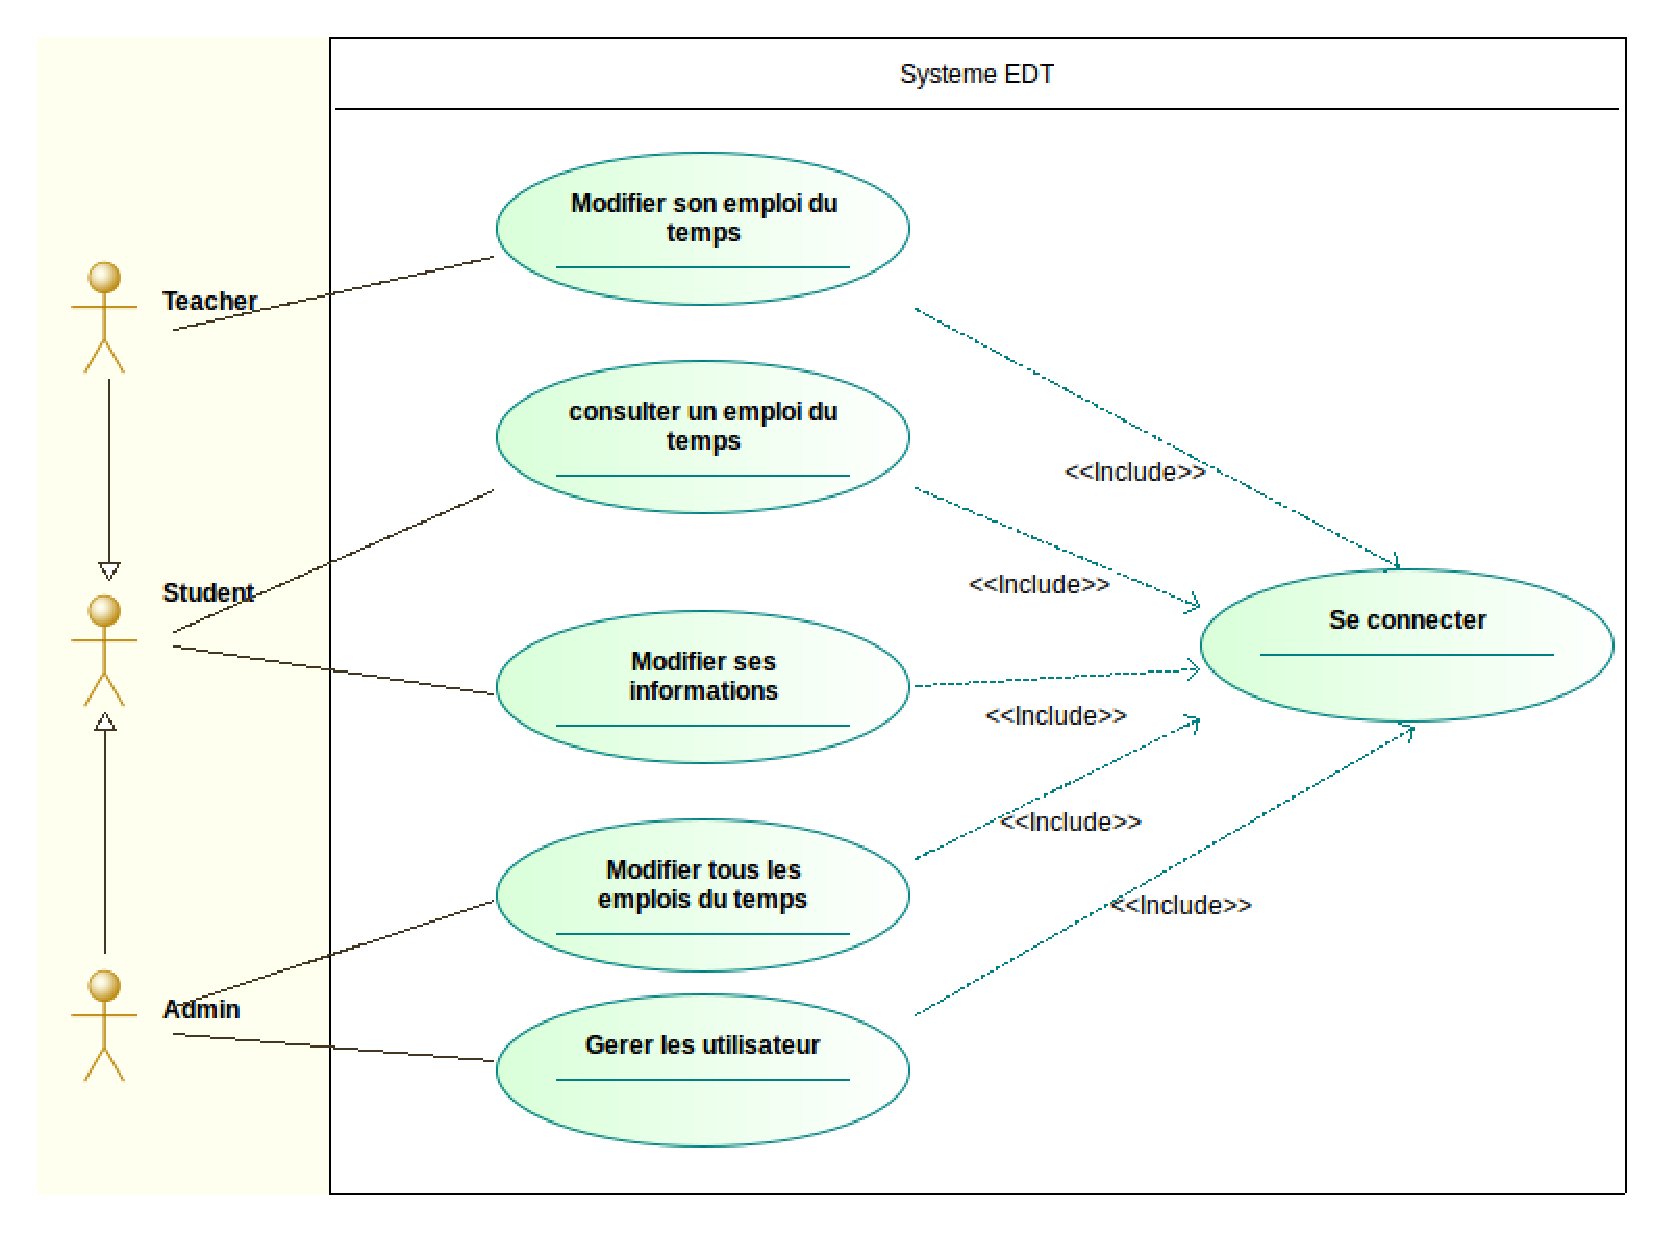
\includegraphics[width=15cm]{fig-diag-use-case-0.eps}}
        \caption{Figure Use Case 0 - niveau principal du diagramme des cas d'utilisation}
        \label{fig-diag-use-case-0}
        \end{figure}
        \begin{itemize}
        \item Consulter un emploi du temps       : Détail figure 3
        \item Changer ses informations           : Détail figure 2
        \item Modifier son emploi du temps       : Détail figure 4
        \item Modifier tous les emplois du temps : Détail figure 4
        \item Gérer les utilisateur              : Détail figure 5
        \item Se connecter                       : Détail figure 1
        \end{itemize}
        %
	\clearpage
        %
        \subsubsection{ Diagrammes de niveau 1}
        %
        \begin{figure}[h]
        \shadowbox{\large\bf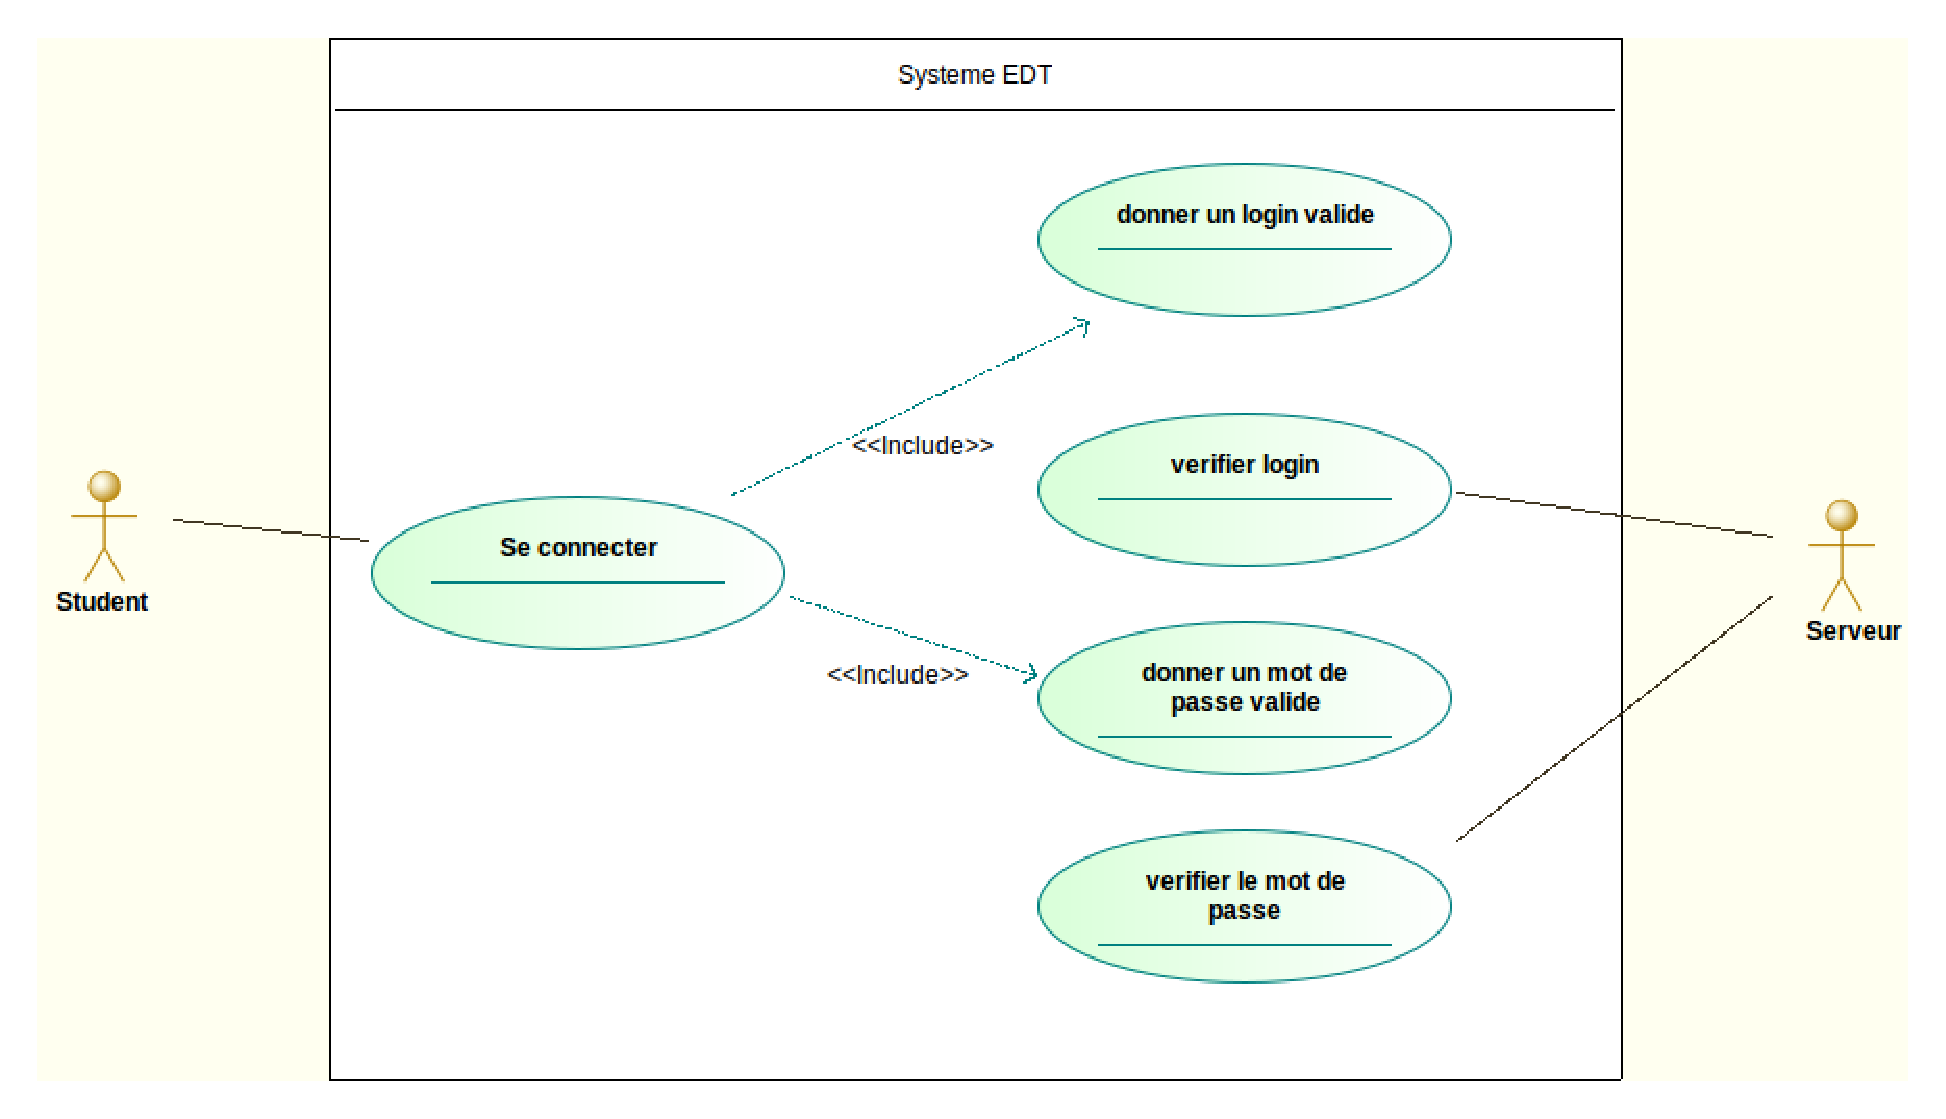
\includegraphics[width=15cm]{fig-diag-use-case-1.eps}}
        \caption{Figure Use Case 1 - Se connecter}
        \label{fig-diag-use-case-1}
        \end{figure}
	%
	\begin{figure}[h]
        \shadowbox{\large\bf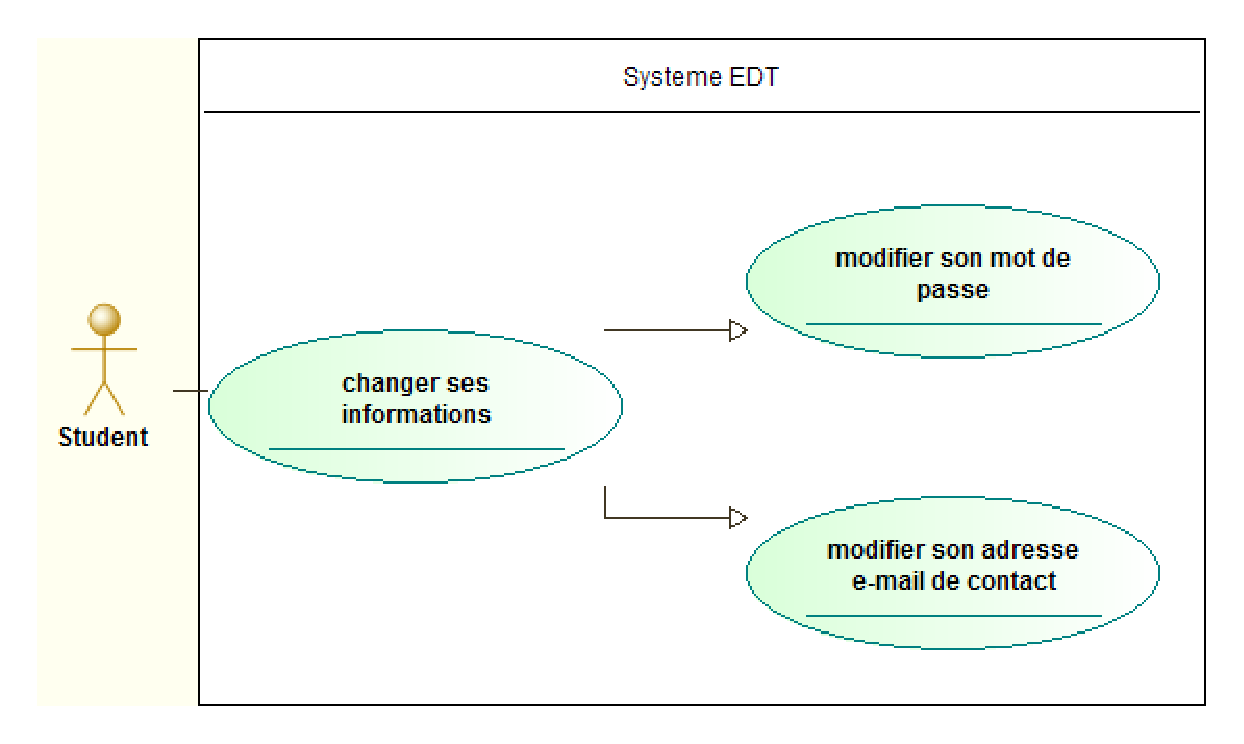
\includegraphics[width=15cm]{fig-diag-use-case-2-2.eps}}
        \caption{Figure Use Case 2 - Changer ses informations}
        \label{fig-diag-use-case-2-2}
        \end{figure}
	\begin{itemize}
        \item Modifier son mot de passe : Détail figure 2-1
        \item Modifier son adresse email de contacte : Détail figure 2-2
        \end{itemize}
	%
        %\begin{figure}[h]
        %\shadowbox{\large\bf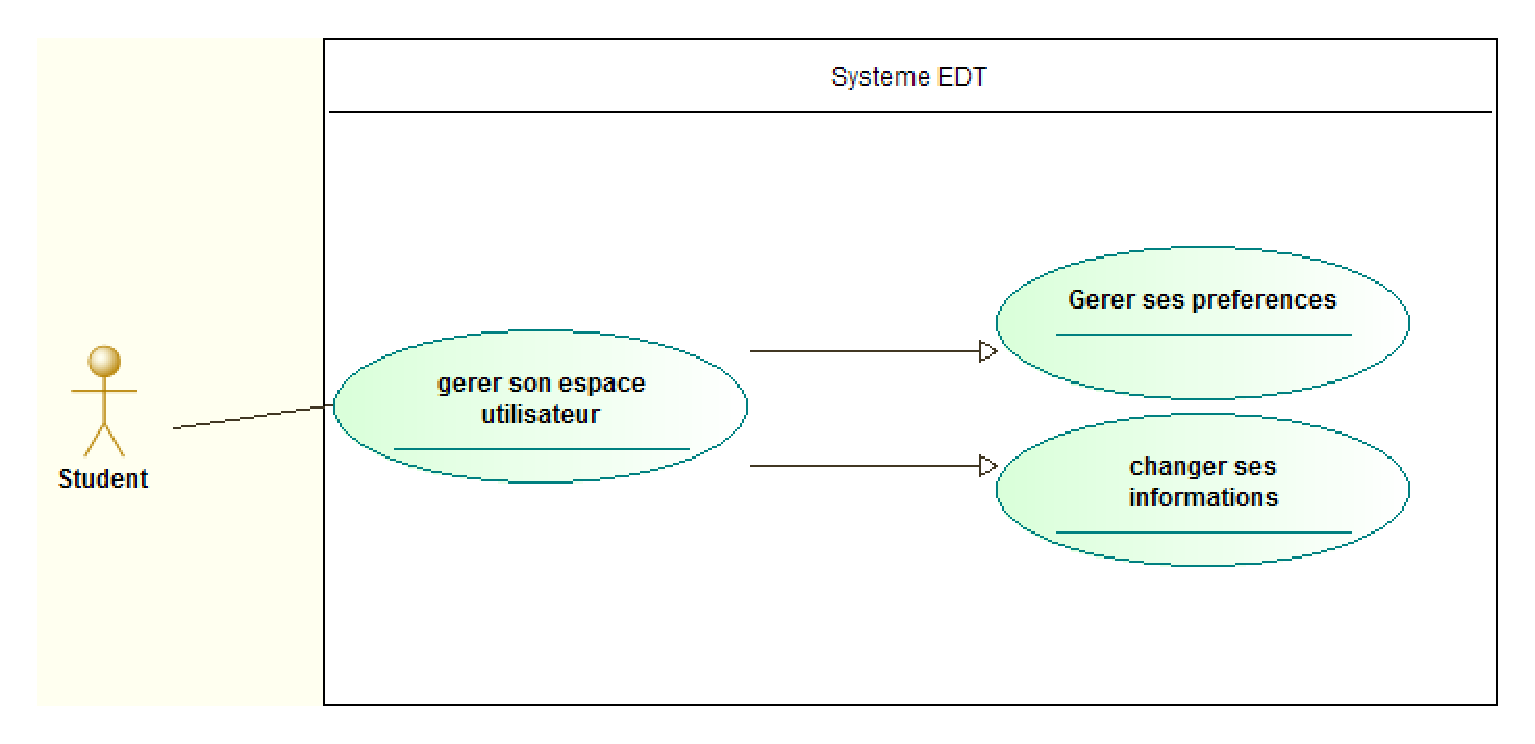
\includegraphics[width=15cm]{fig-diag-use-case-2.eps}}
        %\caption{Figure Use Case 2 - Gérer son espace utilisateur}
        %\label{fig-diag-use-case-2}
        %\end{figure}
        %\begin{itemize}
        %\item Gérer ses préférences : Détail figure 2-1
        %\item Changer ses informations : Détail figure 2-2
        %\end{itemize}
        %
        %\clearpage
        %
        \begin{figure}[h]
        \shadowbox{\large\bf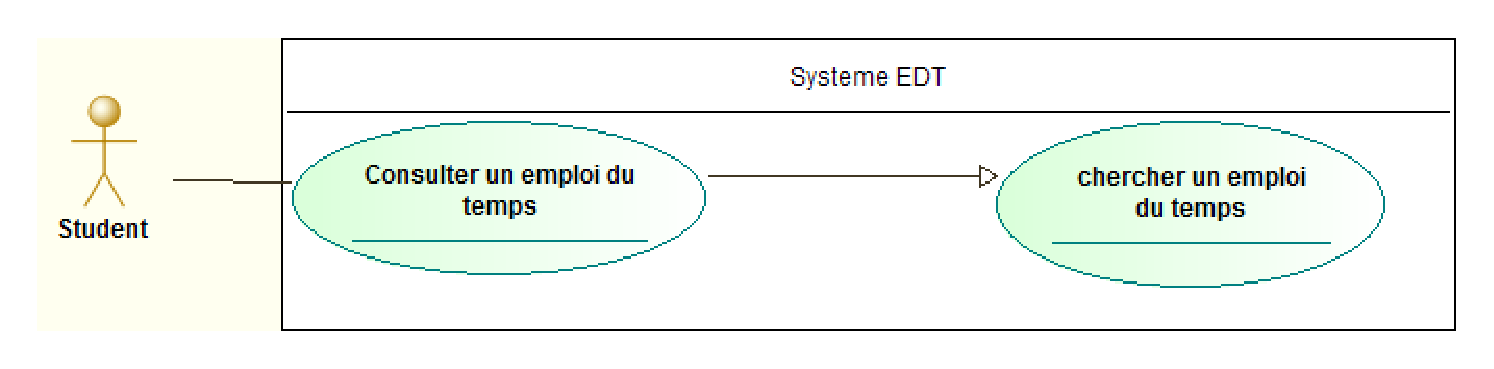
\includegraphics[width=15cm]{fig-diag-use-case-3.eps}}
        \caption{Figure Use Case 3 - Consulter un emploi du temps}
        \label{fig-diag-use-case-3}
        \end{figure}
        \begin{itemize}
        %\item Exporter un emploi du temps : Détail figure 3-1
        \item Chercher un emploi du temps : Détail figure 3-2
        %\item Imprimer un emploi du temps : Détail figure 3-3
        \end{itemize}
	%
	\begin{figure}[h]
        \shadowbox{\large\bf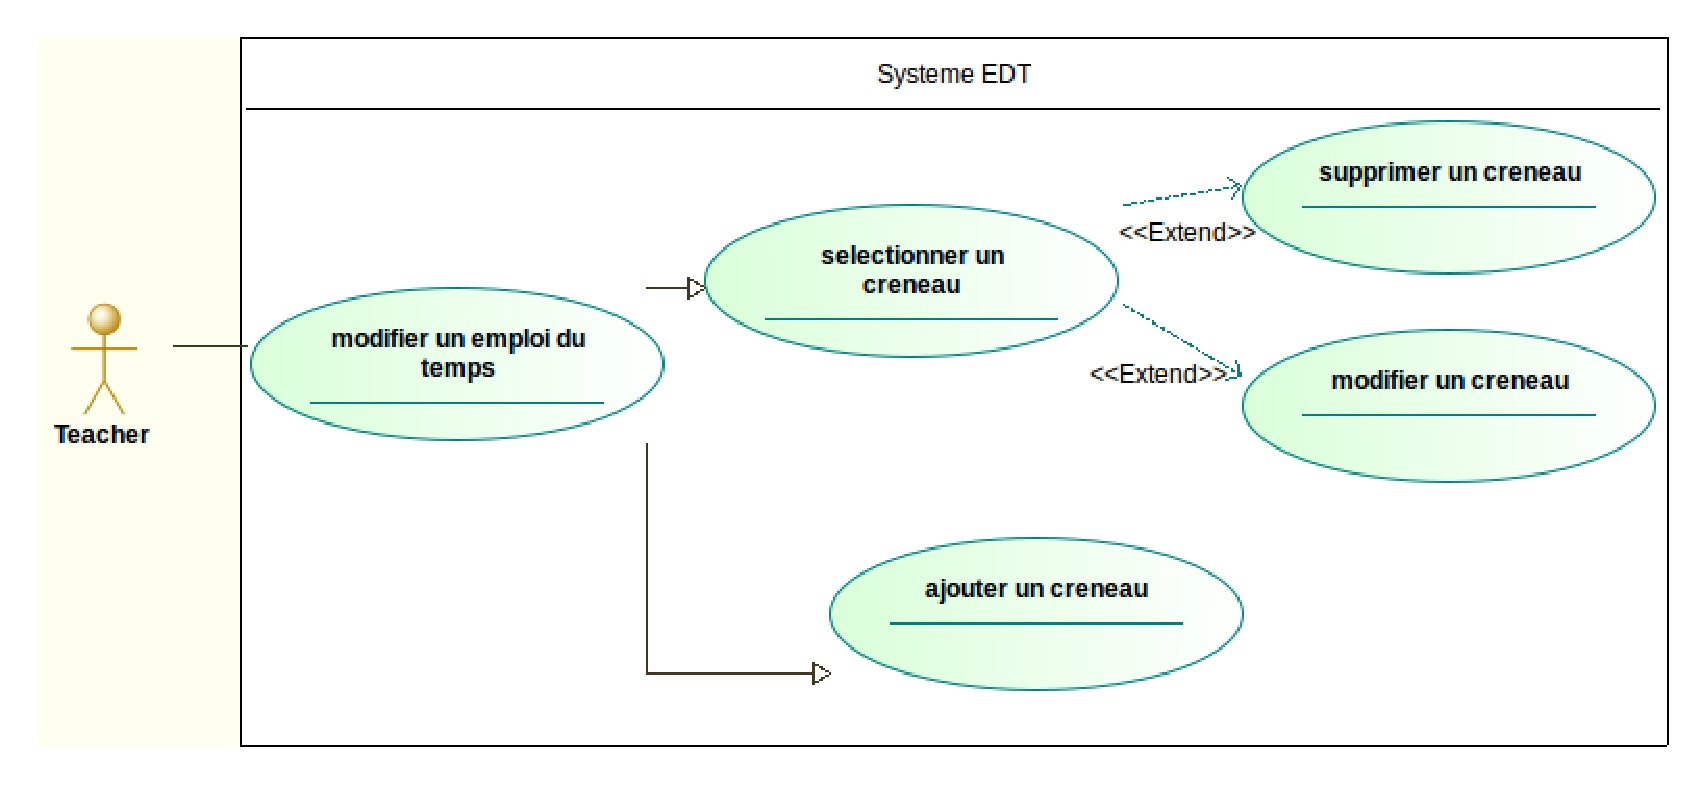
\includegraphics[width=15cm]{fig-diag-use-case-4.eps}}
        \caption{Figure Use Case 4 - Modifier un emploi du temps}
        \label{fig-diag-use-case-4}
        \end{figure}
        \begin{itemize}
        \item Choisir un emploi du temps : Détail figure 4-1
        \item Ajouter un créneau : Détail figure 4-2
        \item Modifier un créneau : Détail figure 4-3
        \end{itemize}
        %
        %\clearpage
        %
	\begin{figure}[h]
        \shadowbox{\large\bf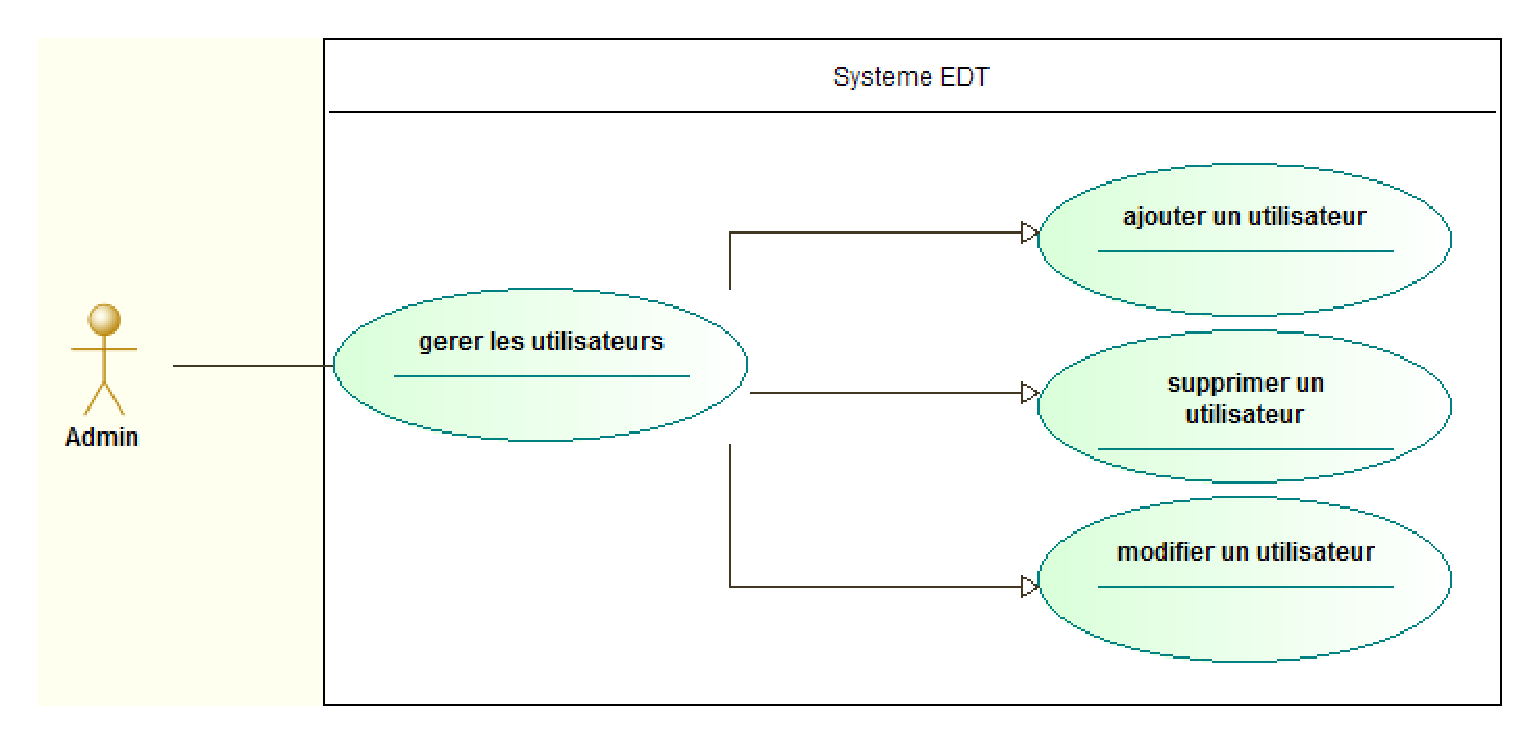
\includegraphics[width=15cm]{fig-diag-use-case-5.eps}}
        \caption{Figure Use Case 5 - Gérer les utilisateur}
        \label{fig-diag-use-case-5}
        \end{figure}
        \begin{itemize}
        \item Ajouter un utilisateur : Détail 5-1
        \item Modifier un utilisateur : Détail 5-2
        \end{itemize}
        %
        \clearpage
	%
	%\begin{figure}[h]
        %\shadowbox{\large\bf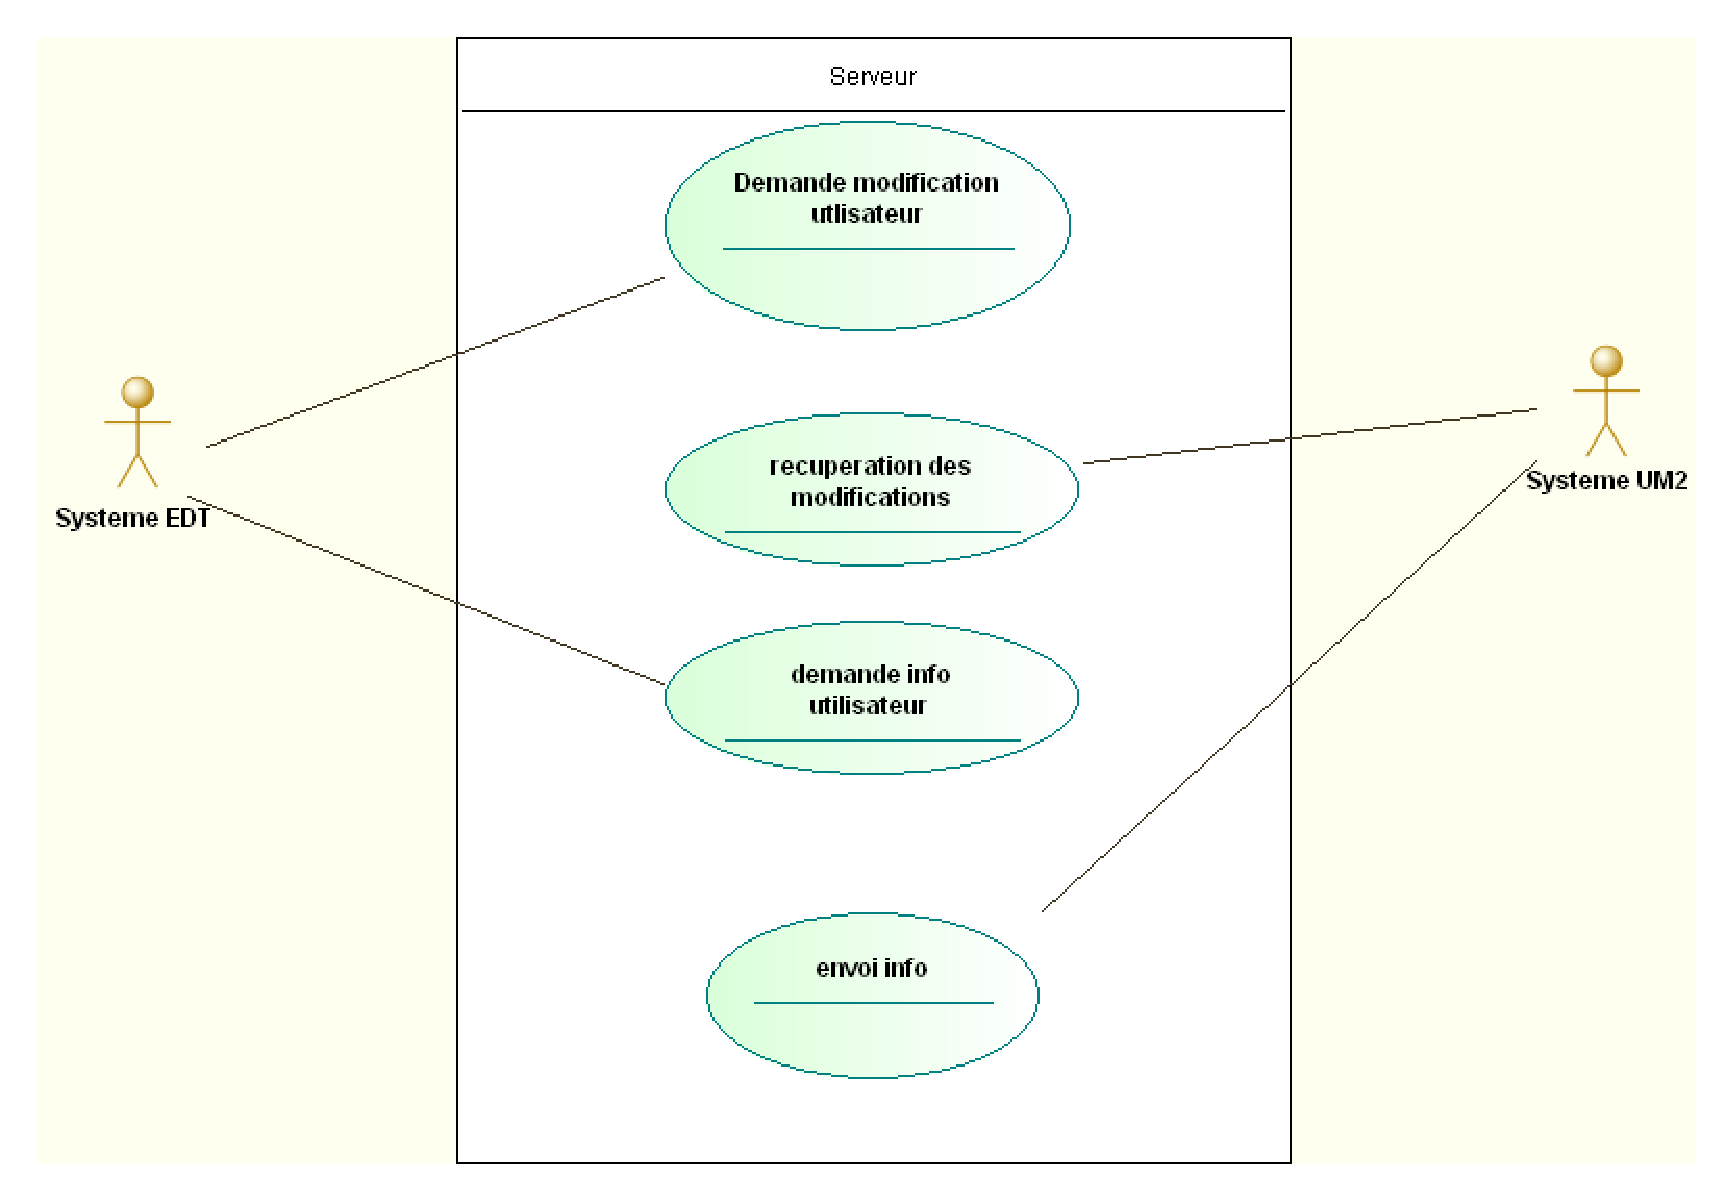
\includegraphics[width=15cm]{fig-diag-use-case-6.eps}}
        %\caption{Figure Use Case 6 - Système Serveur échange de donnée}
        %\label{fig-diag-use-case-6}
        %\end{figure}
        %Gestion et partages des données contenu dans la base de donnée du système EDT et la base de donnée de l'UM2.
	%
	%\begin{figure}[h]
        %\shadowbox{\large\bf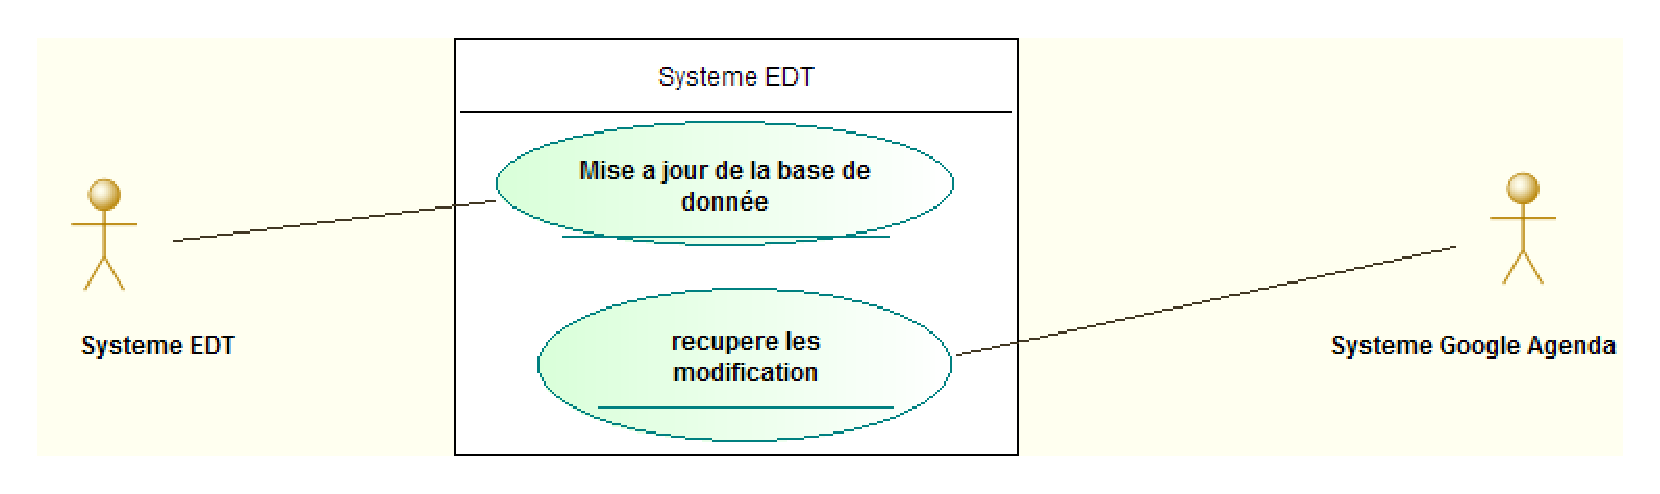
\includegraphics[width=15cm]{fig-diag-use-case-7.eps}}
        %\caption{Figure Use Case 7 - Système Serveur échange avec Google Agenda}
        %\label{fig-diag-use-case-7}
        %\end{figure}
        %Envoi des données du système EDT vers le système Google Agenda pour exporter un emploi du temps.
	%
	\clearpage
	%
        \subsubsection{ Diagrammes de niveau 2}
        %
	\begin{figure}[h]
        \shadowbox{\large\bf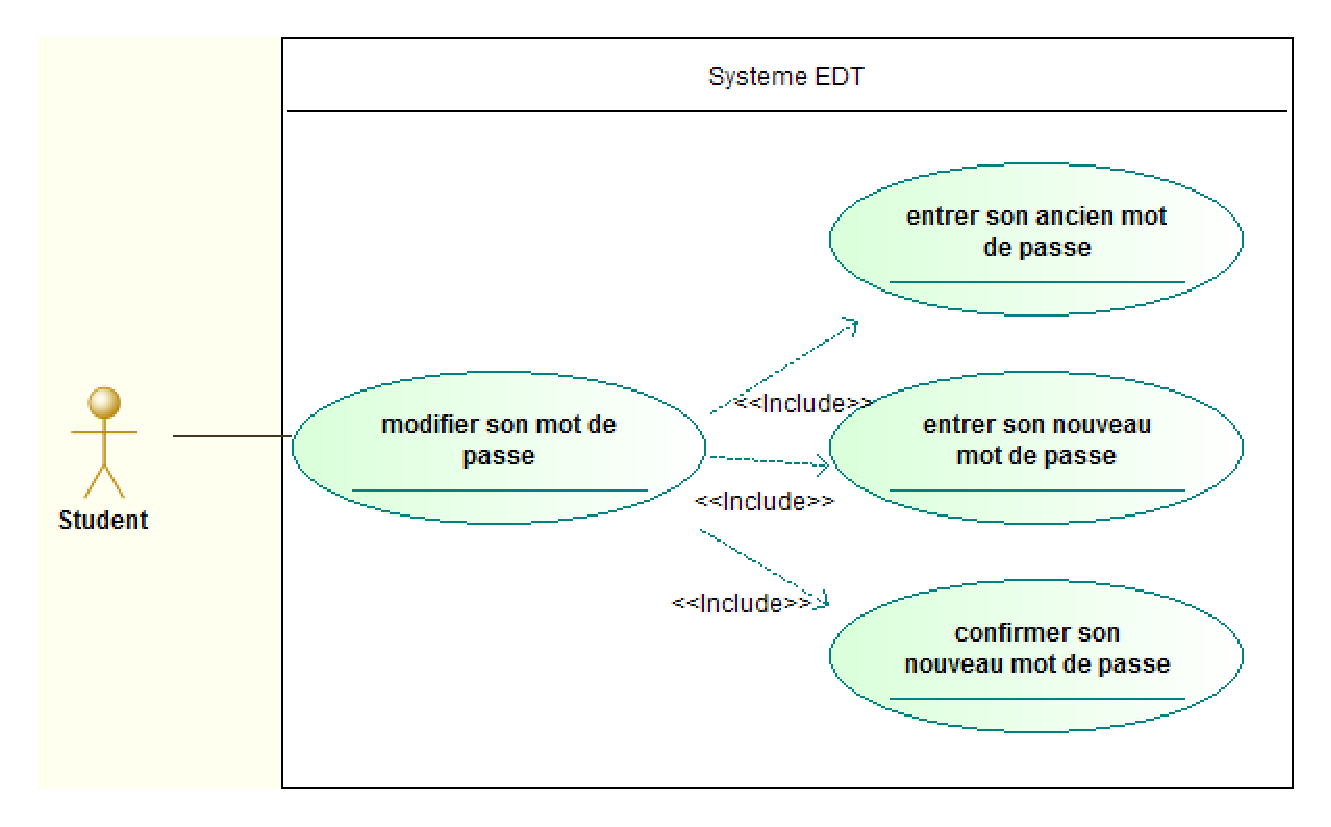
\includegraphics[width=15cm]{fig-diag-use-case-2-2-1.eps}}
        \caption{Figure Use Case 2.1 - Modifier son mot de passe}
        \label{fig-diag-use-case-2-2-1}
        \end{figure}
	%
	\begin{figure}[h]
        \shadowbox{\large\bf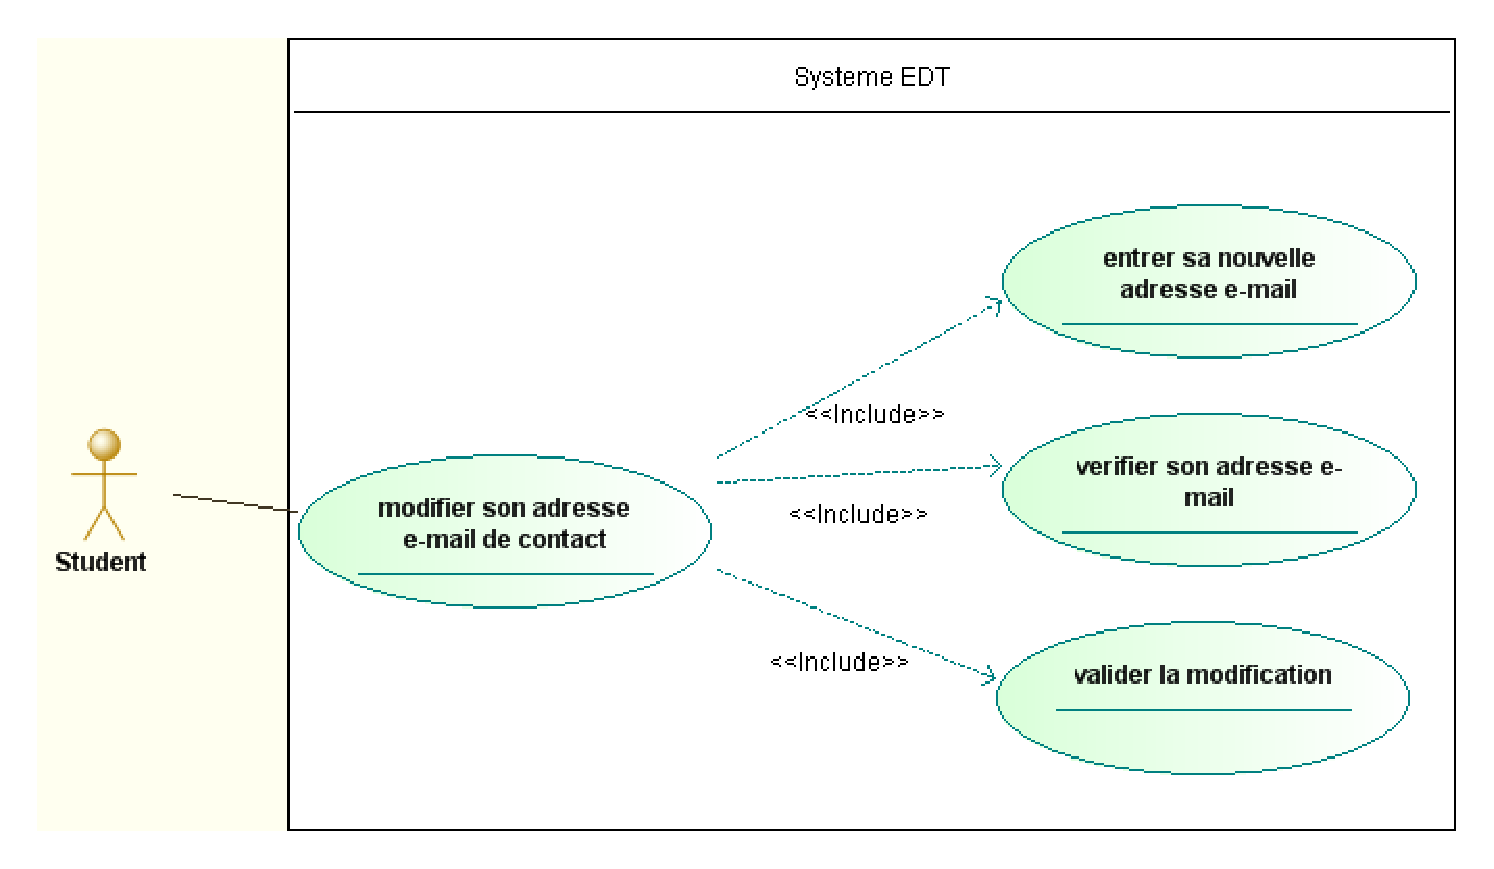
\includegraphics[width=15cm]{fig-diag-use-case-2-2-2.eps}}
        \caption{Figure Use Case 2.2 - Modifier son adresse email de contact}
        \label{fig-diag-use-case-2-2-2}
        \end{figure}
	%
	\clearpage
	%
        %\begin{figure}[h]
        %\shadowbox{\large\bf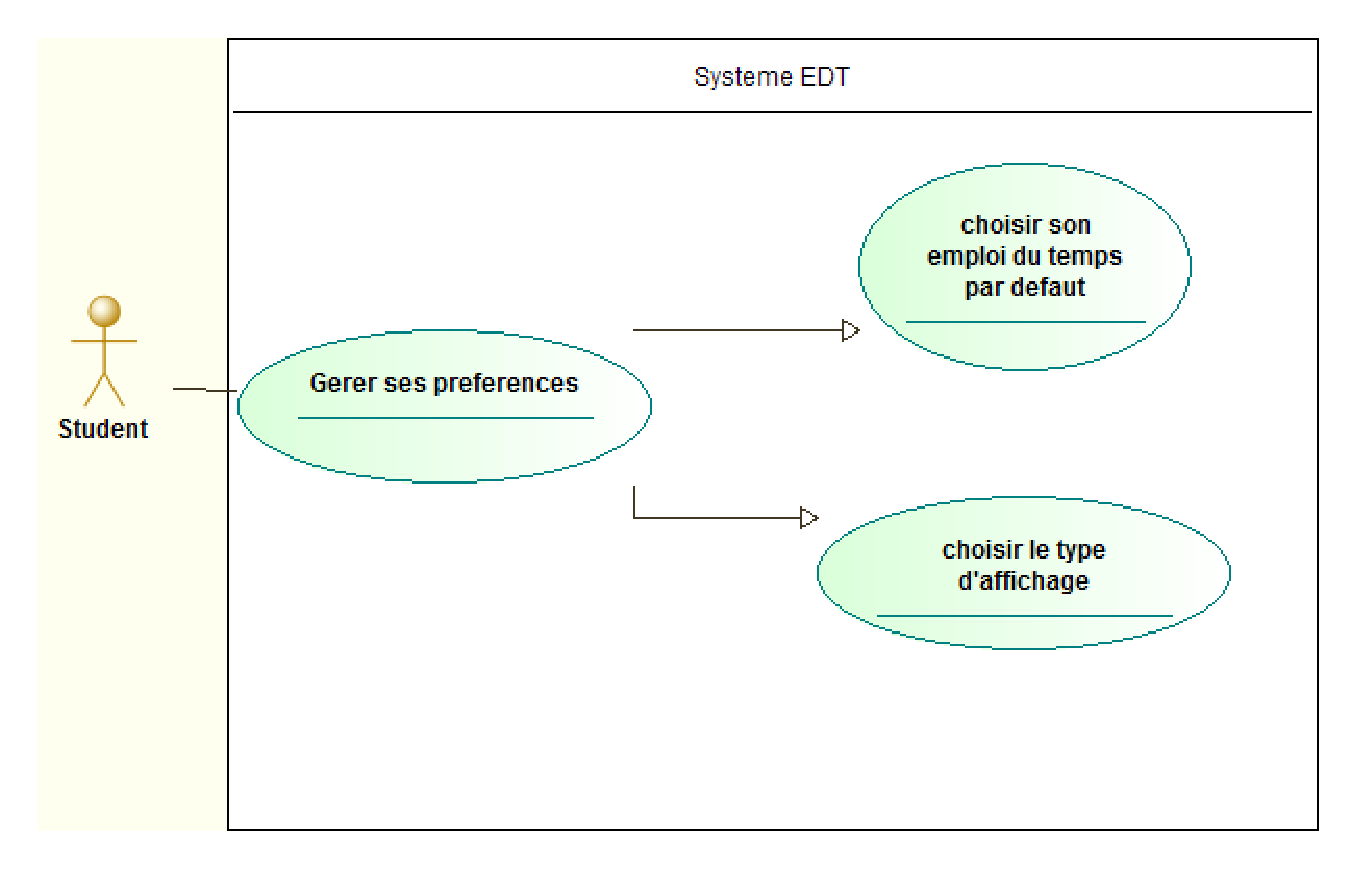
\includegraphics[width=15cm]{fig-diag-use-case-2-1.eps}}
        %\caption{Figure Use Case 2.1 - Gérer ses préférences}
        %\label{fig-diag-use-case-2-1}
        %\end{figure}
        %\begin{itemize}
        %\item Choisir son emploi du temps par défaut : Détail figure 2-1-1
        %\item Choisir le type d'affichage : Détail figure 2-1-2
        %\end{itemize}
        %\clearpage
	%
	%\begin{figure}[h]
        %\shadowbox{\large\bf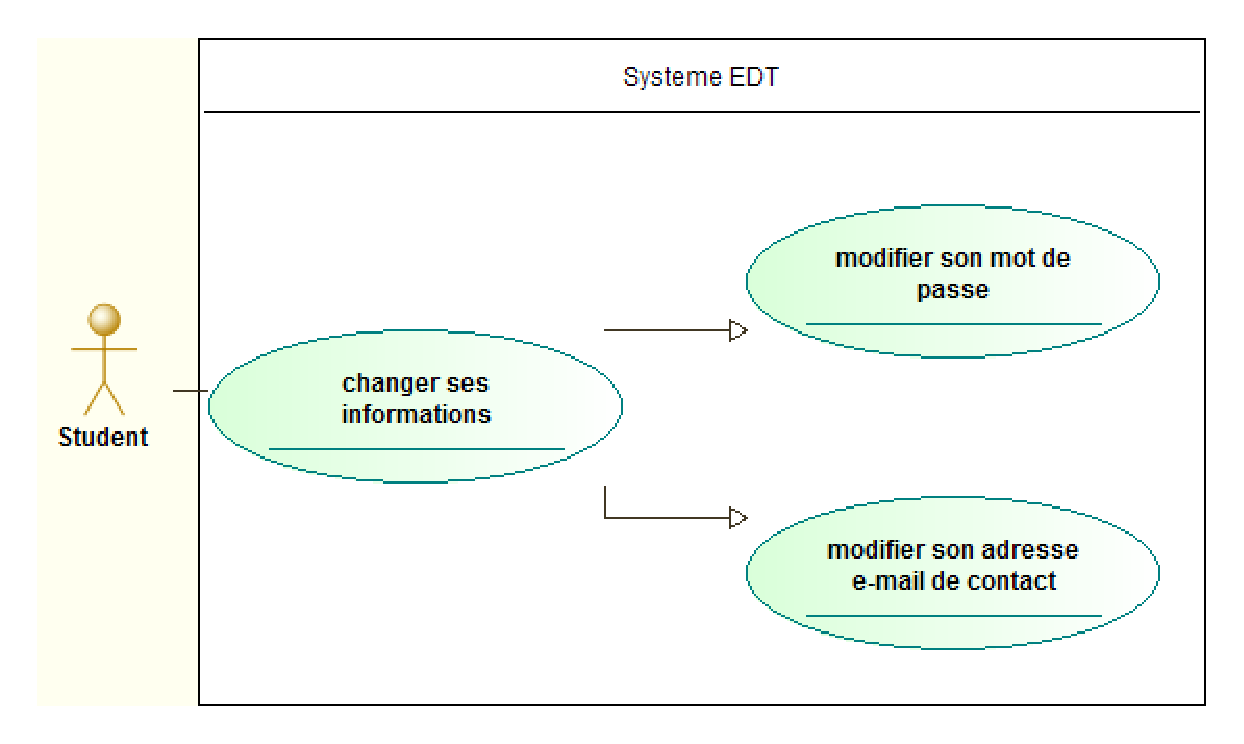
\includegraphics[width=15cm]{fig-diag-use-case-2-2.eps}}
        %\caption{Figure Use Case 2.2 - Changer ses informations}
        %\label{fig-diag-use-case-2-2}
        %\end{figure}
        %\begin{itemize}
        %\item Modifier son mot de passe : Détail figure 2-2-1
        %\item Modifier son adresse email de contacte : Détail figure 2-2-2
        %\end{itemize}
        %
        %\clearpage
	%
	%\begin{figure}[h]
        %\shadowbox{\large\bf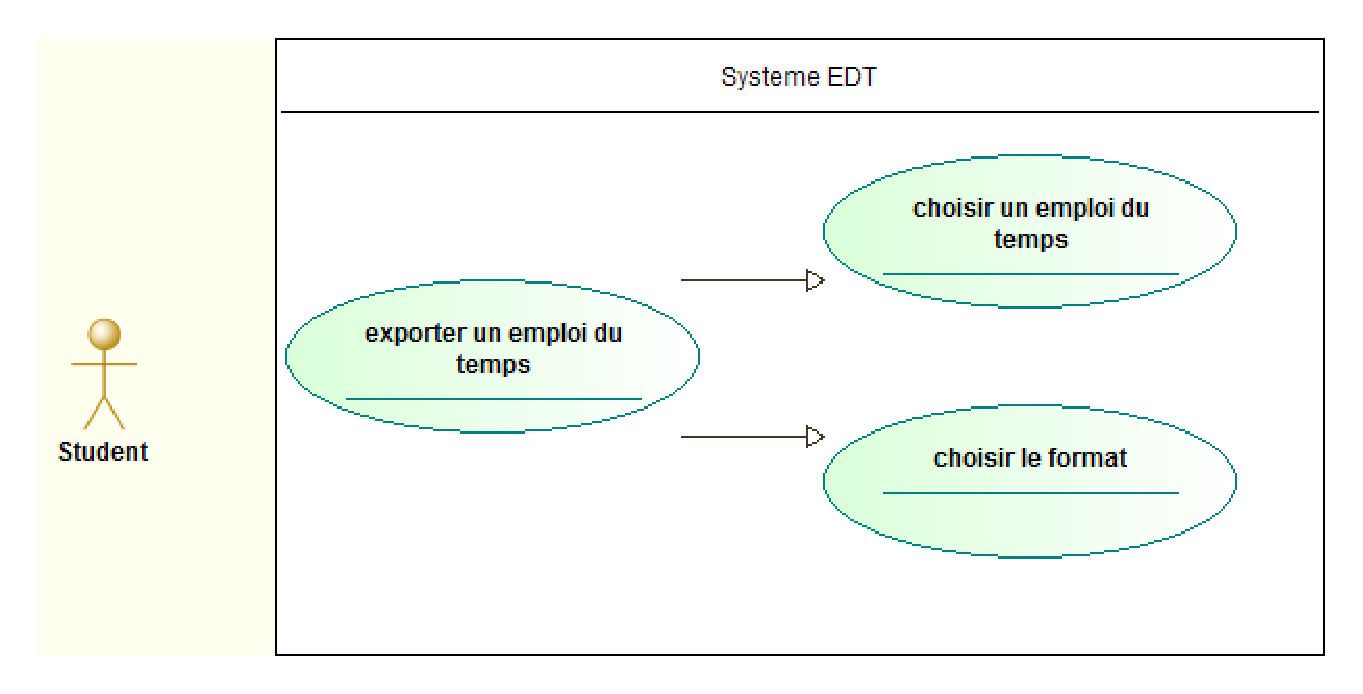
\includegraphics[width=15cm]{fig-diag-use-case-3-1.eps}}
        %\caption{Figure Use Case 3.1 - Exporter un emploi du temps}
        %\label{fig-diag-use-case-3-1}
        %\end{figure}
        %\begin{itemize}
        %\item Choisir un emploi du temps : Détail figure 4-1
        %\item Choisir le format : Détail figure 3-1-2
        %\end{itemize}
	%
	\begin{figure}[h]
        \shadowbox{\large\bf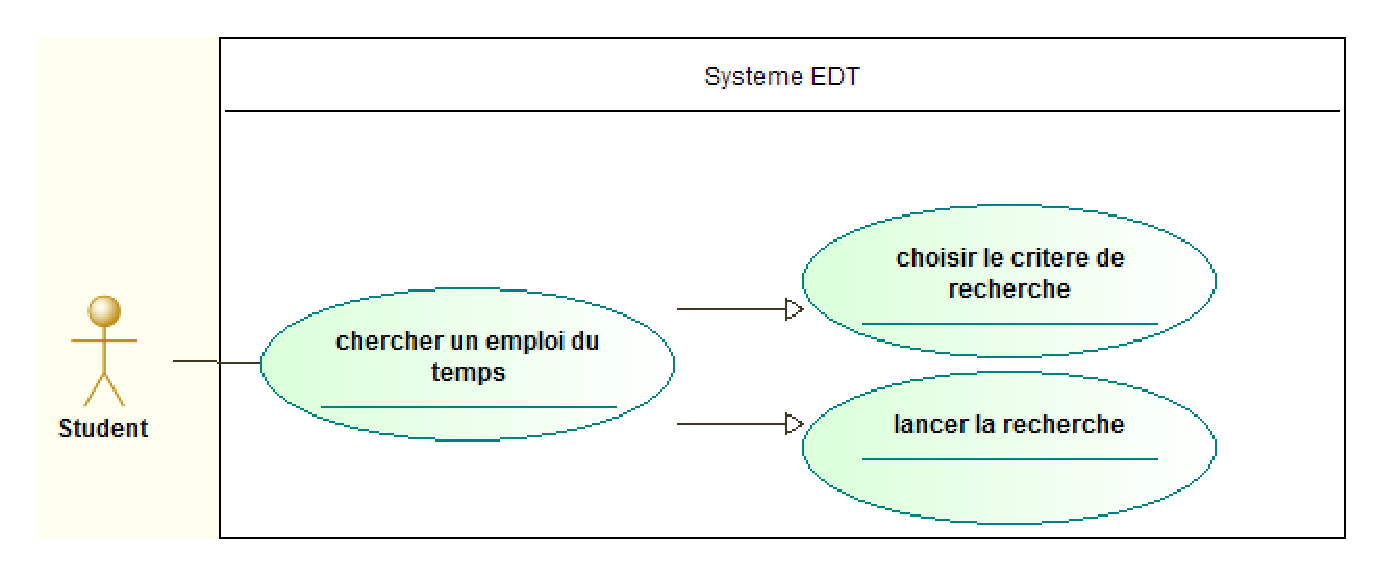
\includegraphics[width=15cm]{fig-diag-use-case-3-2.eps}}
        \caption{Figure Use Case 3.2 - Chercher un emploi du temps}
        \label{fig-diag-use-case-3-2}
        \end{figure}
	%
	%\clearpage
	%
	%\begin{figure}[h]
        %\shadowbox{\large\bf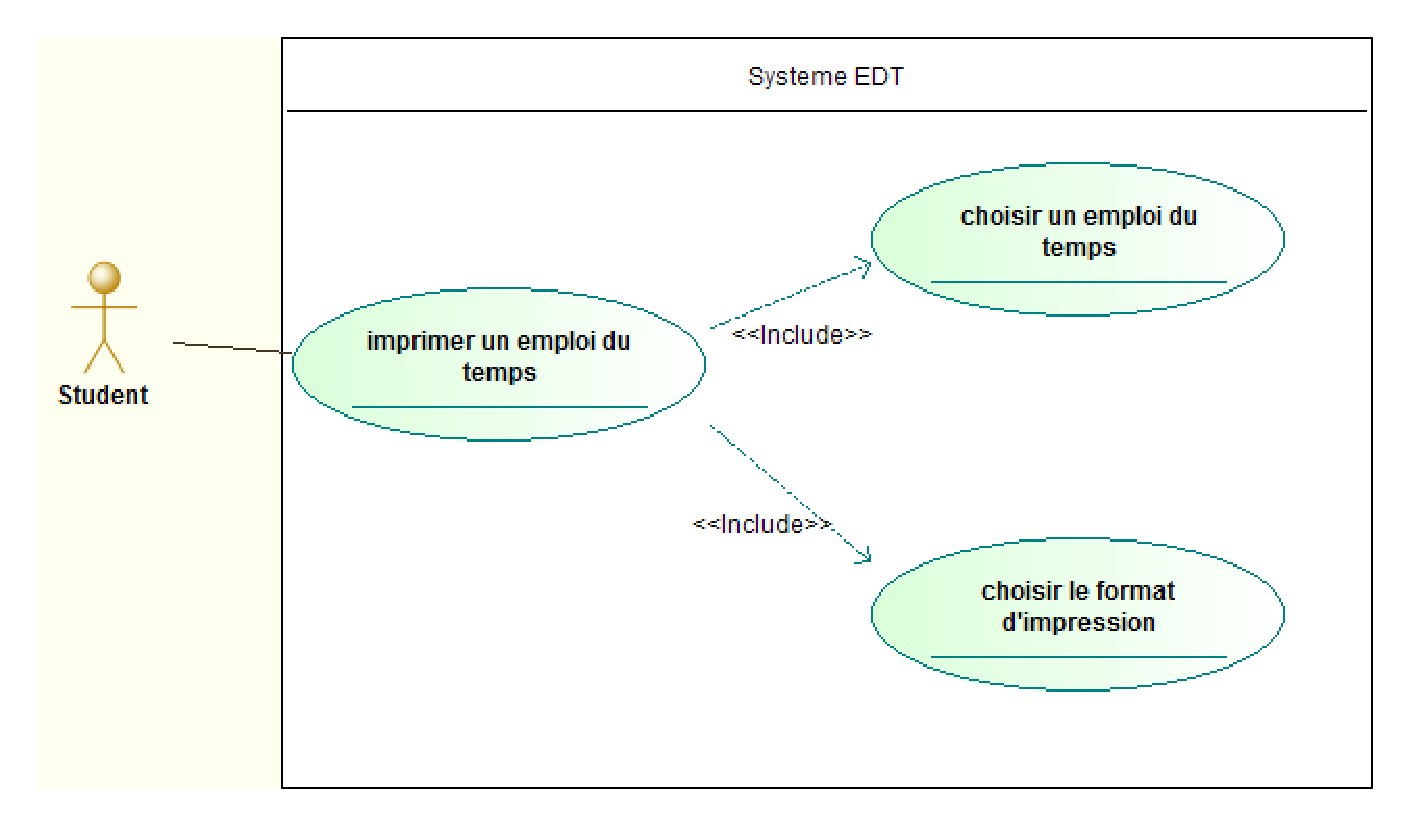
\includegraphics[width=15cm]{fig-diag-use-case-3-3.eps}}
        %\caption{Figure Use Case 3.3 - Imprimer un emploi du temps}
        %\label{fig-diag-use-case-3-3}
        %\end{figure}
        %\begin{itemize}
        %\item Choisir un emploi du temps : Détail figure 4-1
        %\end{itemize}
        %
	%\clearpage
        %
	\begin{figure}[h]
        \shadowbox{\large\bf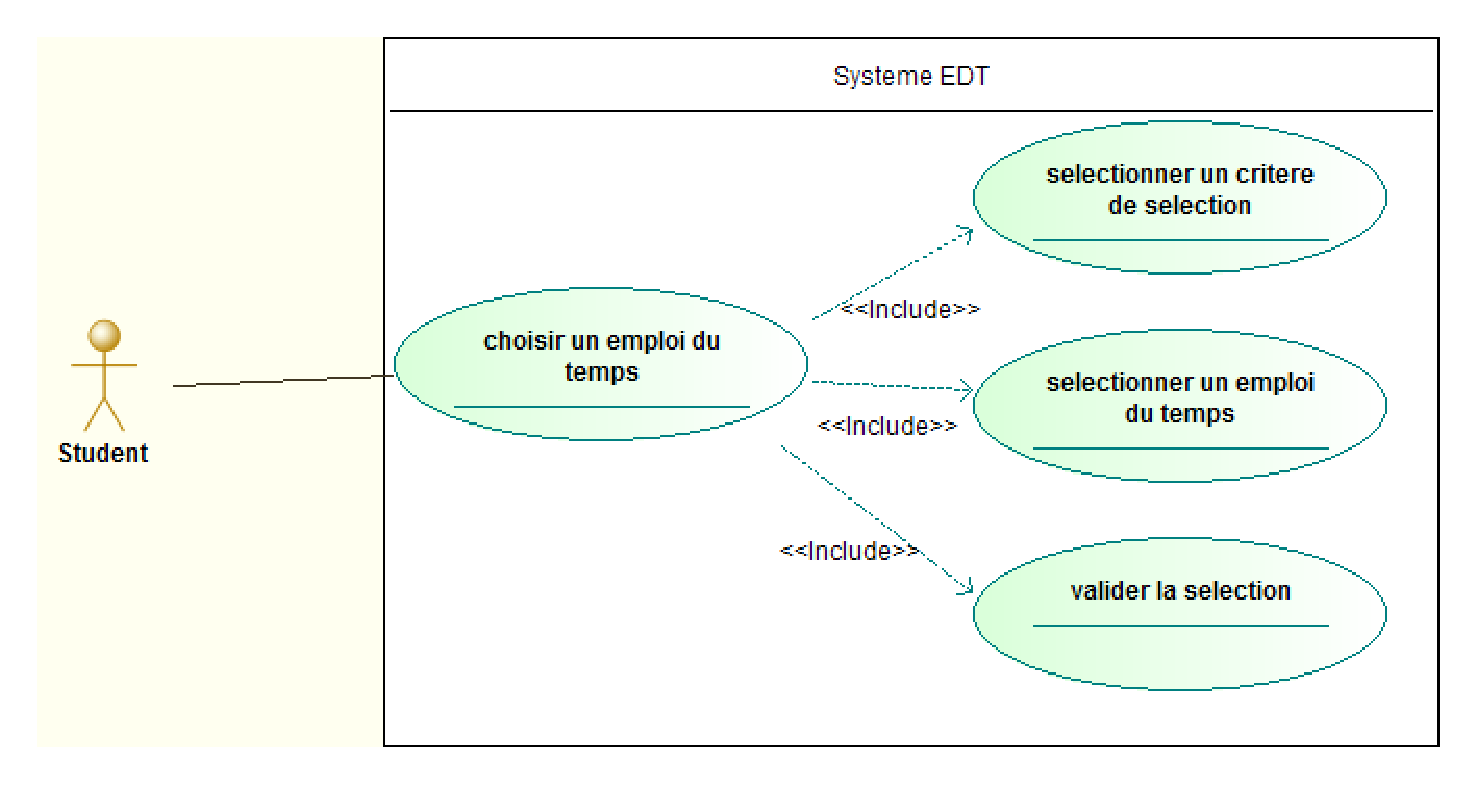
\includegraphics[width=15cm]{fig-diag-use-case-4-1.eps}}
        \caption{Figure Use Case 4.1 - Choisir un emploi du temps}
        \label{fig-diag-use-case-4-1}
        \end{figure}
        \begin{itemize}
        \item Séléctionner un critère de séléction : Détail figure 4-1-1
        \end{itemize}
	%
	\clearpage
        %
	\begin{figure}[h]
        \shadowbox{\large\bf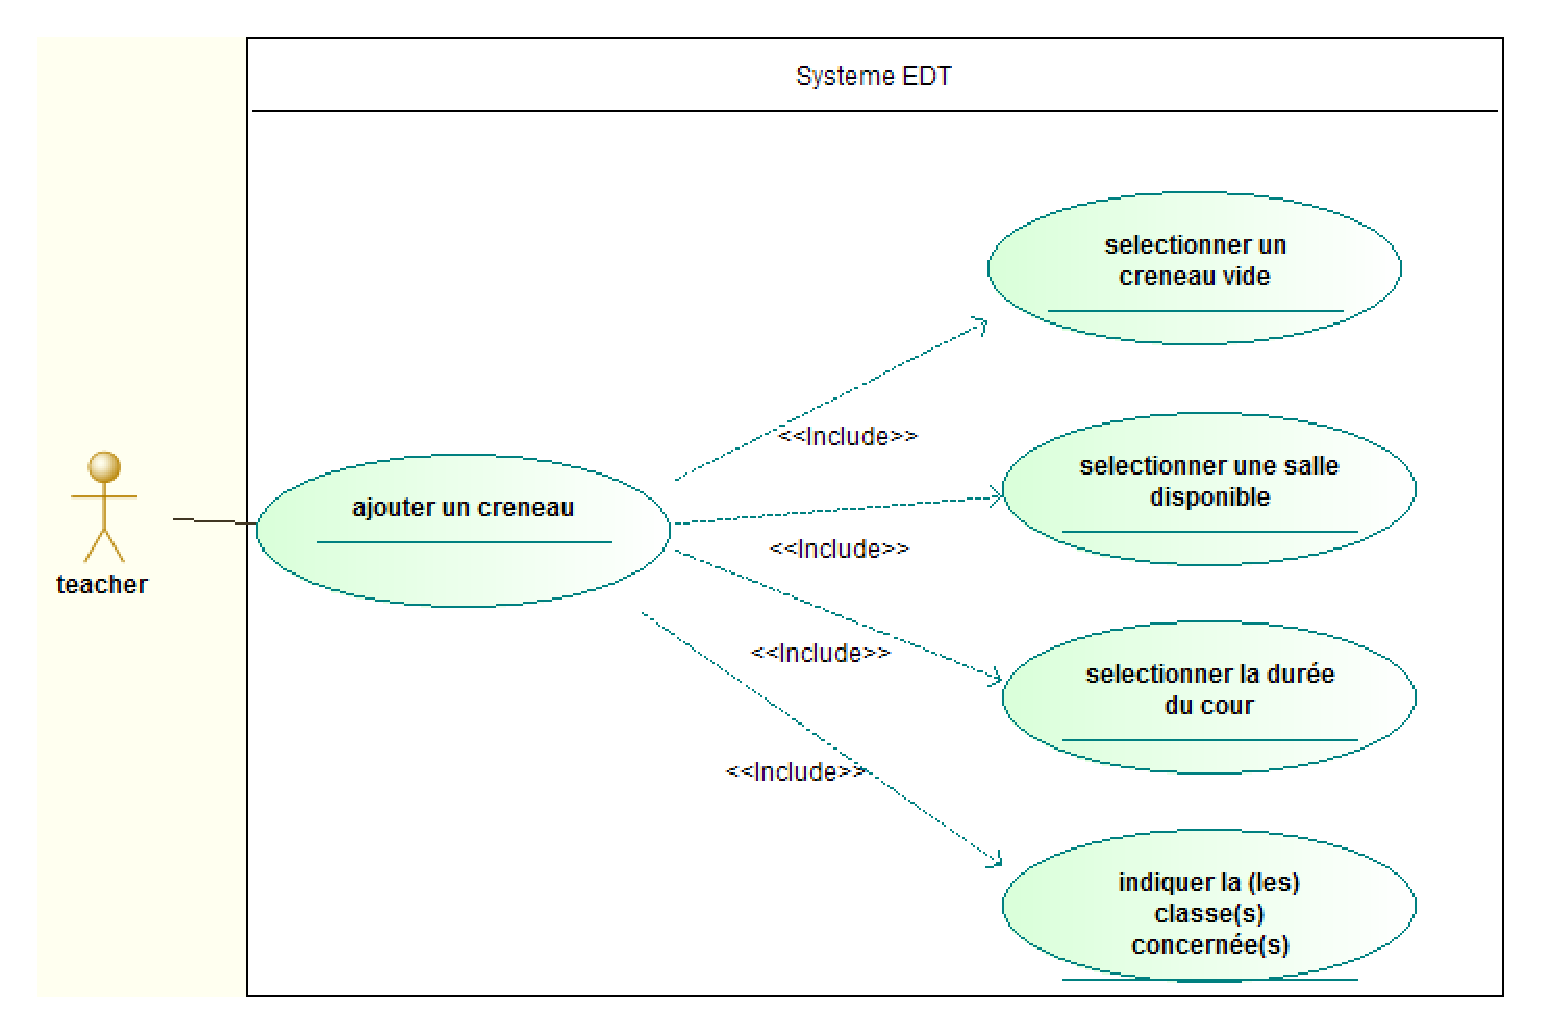
\includegraphics[width=15cm]{fig-diag-use-case-4-2.eps}}
        \caption{Figure Use Case 4.2 - Ajouter un créneau}
        \label{fig-diag-use-case-4-2}
        \end{figure}
	%
	\begin{figure}[h]
        \shadowbox{\large\bf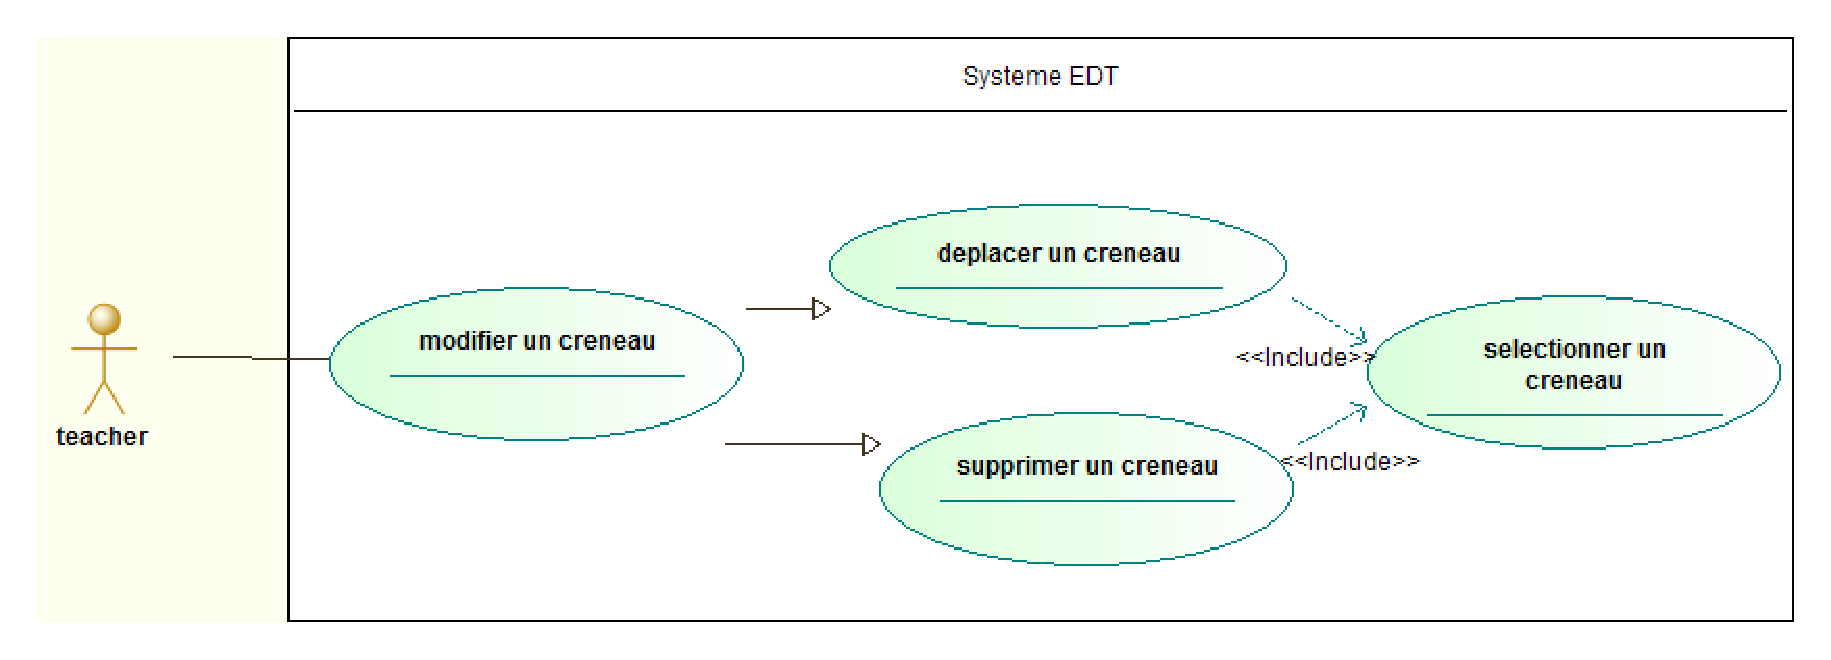
\includegraphics[width=15cm]{fig-diag-use-case-4-3.eps}}
        \label{fig-diag-use-case-4-3}
        \caption{Figure Use Case 4.3 - Modifier un créneau}
        \end{figure}
        %
        \clearpage
	%
	\begin{figure}[!h]
        \shadowbox{\large\bf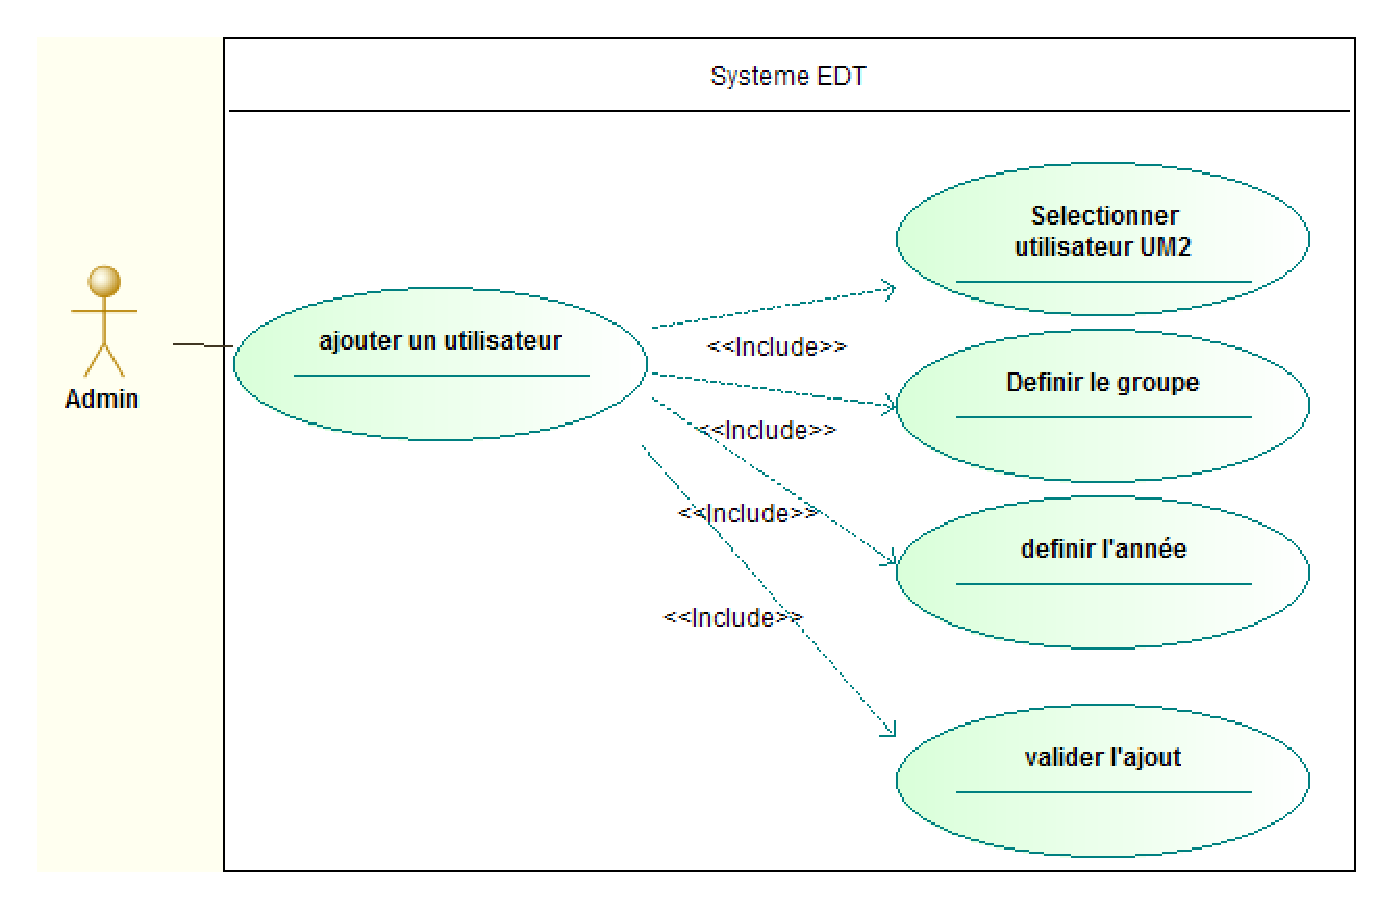
\includegraphics[width=15cm]{fig-diag-use-case-5-1.eps}}
        \caption{Figure Use Case 5.1 - Ajouter un utilisateur}
        \label{fig-diag-use-case-5-1}
        \end{figure}
	%
	\begin{figure}[!h]
        \shadowbox{\large\bf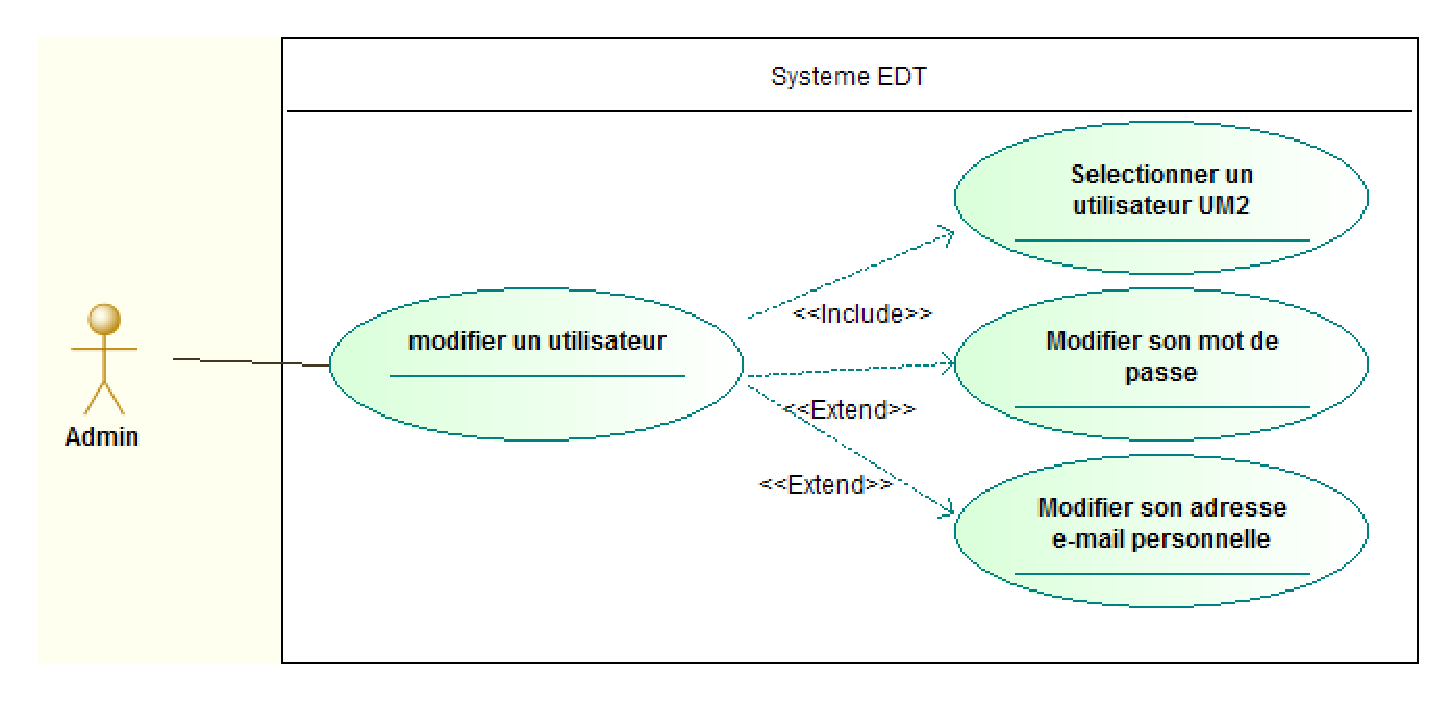
\includegraphics[width=15cm]{fig-diag-use-case-5-2.eps}}
        \caption{Figure Use Case 5.2 - Modifier un utilisateur}
        \label{fig-diag-use-case-5-2}
        \end{figure}
	%
	\clearpage
	%
	\subsubsection{ Diagrammes de niveau 3}
	%
	%\begin{figure}[h]
        %\shadowbox{\large\bf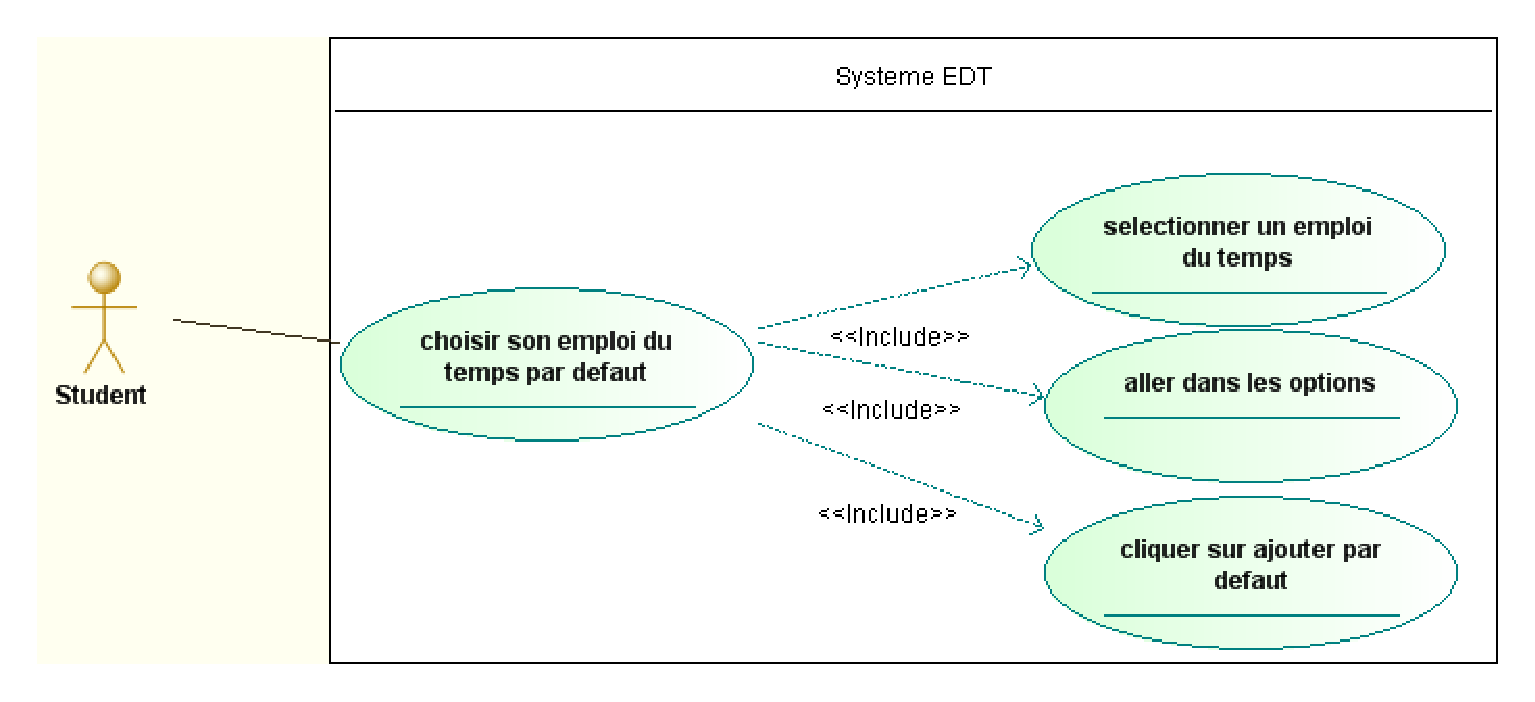
\includegraphics[width=15cm]{fig-diag-use-case-2-1-1.eps}}
        %\caption{Figure Use Case 2.1.1 - Choisir son emploi du temps par défaut}
        %\label{fig-diag-use-case-2-1-1}
        %\end{figure}
	%
	%\begin{figure}[h]
        %\shadowbox{\large\bf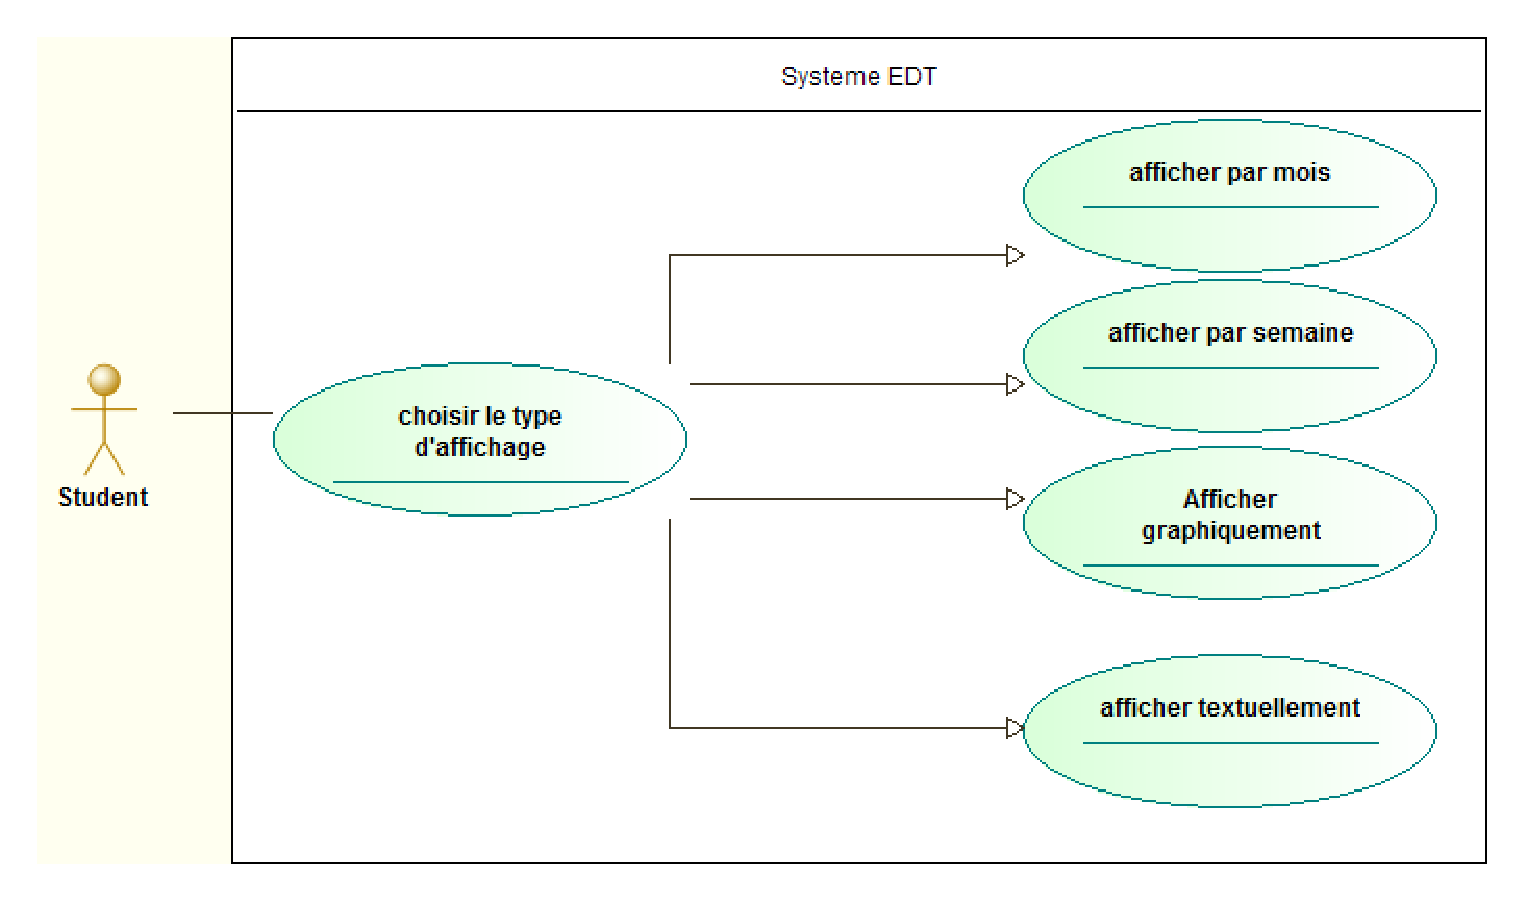
\includegraphics[width=15cm]{fig-diag-use-case-2-1-2.eps}}
        %\caption{Figure Use Case 2.1.2 - Choisir le type d'affichage}
        %\label{fig-diag-use-case-2-1-2}
        %\end{figure}
        %
	%\clearpage
	%
	%\begin{figure}[h]
        %\shadowbox{\large\bf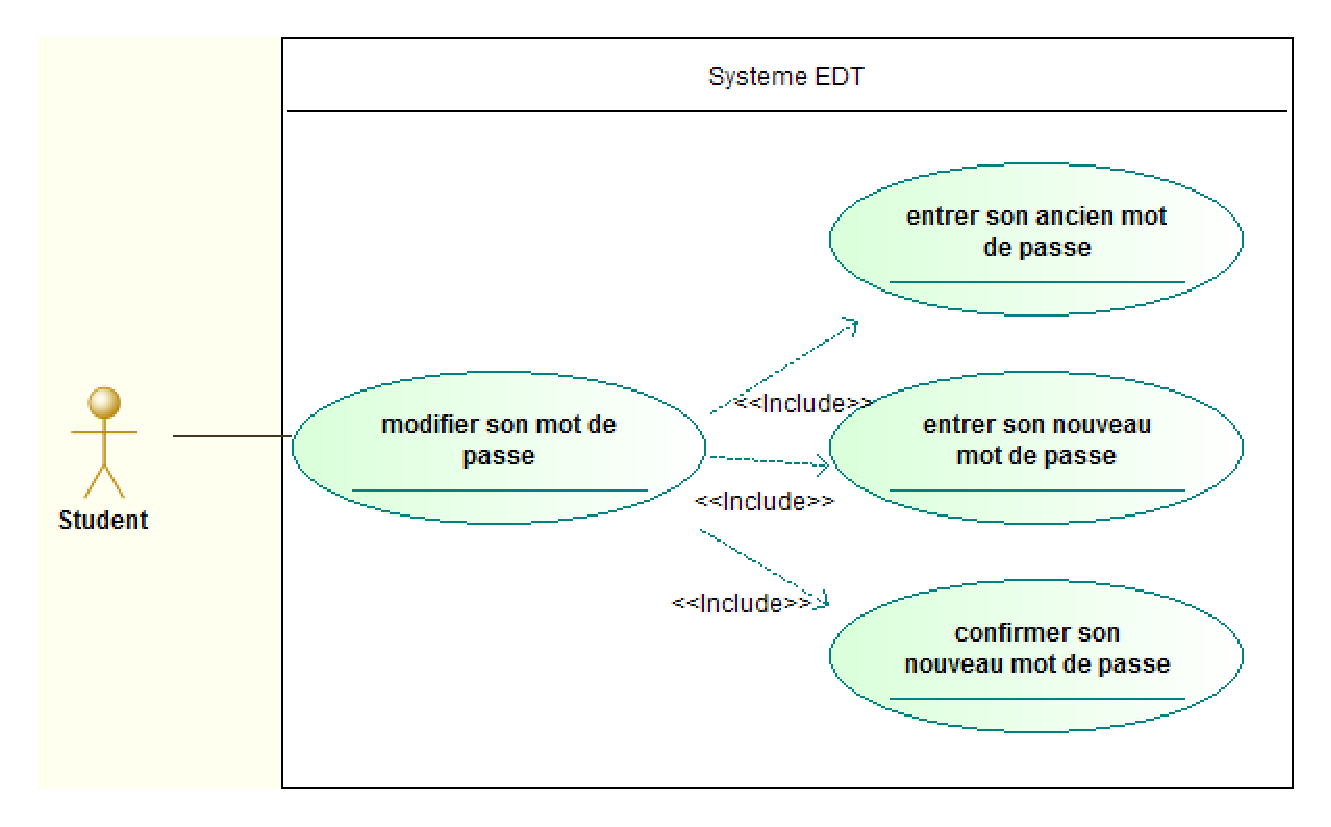
\includegraphics[width=15cm]{fig-diag-use-case-2-2-1.eps}}
        %\caption{Figure Use Case 2.2.1 - Modifier son mot de passe}
        %\label{fig-diag-use-case-2-2-1}
        %\end{figure}
	%
	%\begin{figure}[h]
        %\shadowbox{\large\bf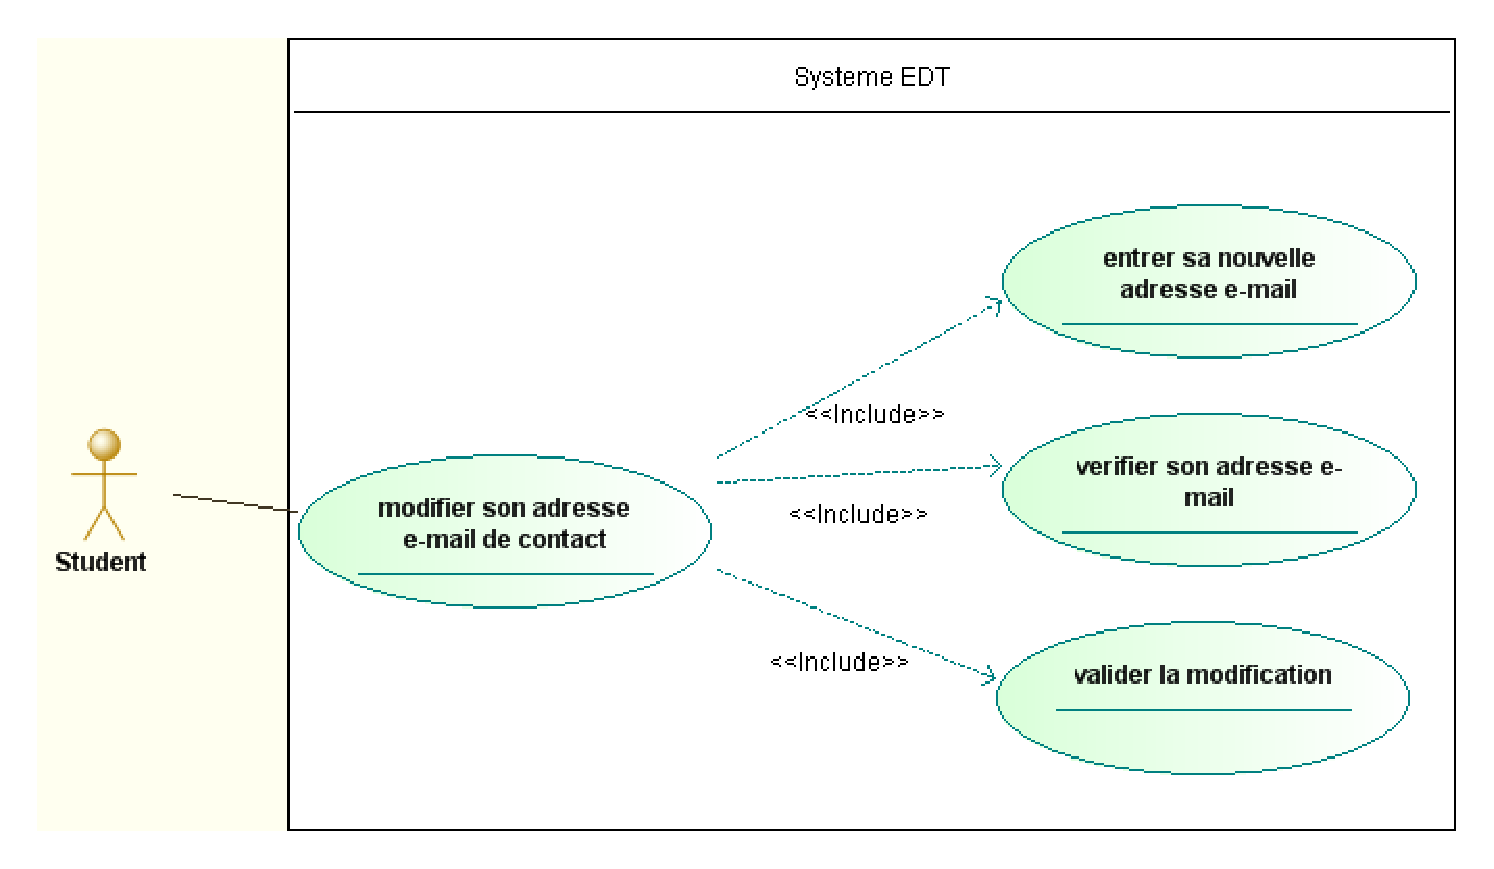
\includegraphics[width=15cm]{fig-diag-use-case-2-2-2.eps}}
        %\caption{Figure Use Case 2.2.2 - Modifier son adresse email de contact}
        %\label{fig-diag-use-case-2-2-2}
        %\end{figure}
	%
	%\clearpage
	%
	%\begin{figure}[h]
        %\shadowbox{\large\bf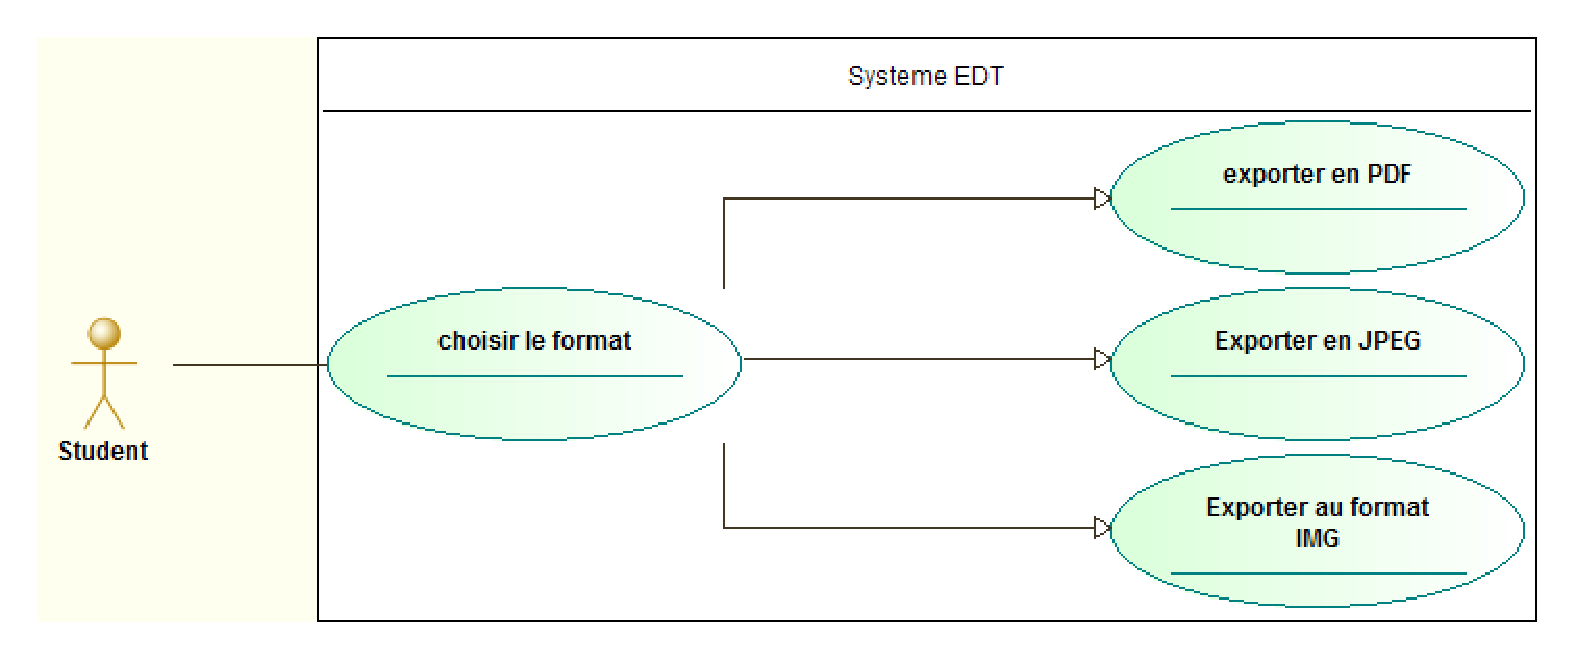
\includegraphics[width=15cm]{fig-diag-use-case-3-1-2.eps}}
        %\caption{Figure Use Case 3.1.2 - Choisir le format}
        %\label{fig-diag-use-case-3-1-2}
        %\end{figure}
	%
	%\clearpage
	%
	\begin{figure}[h]
        \shadowbox{\large\bf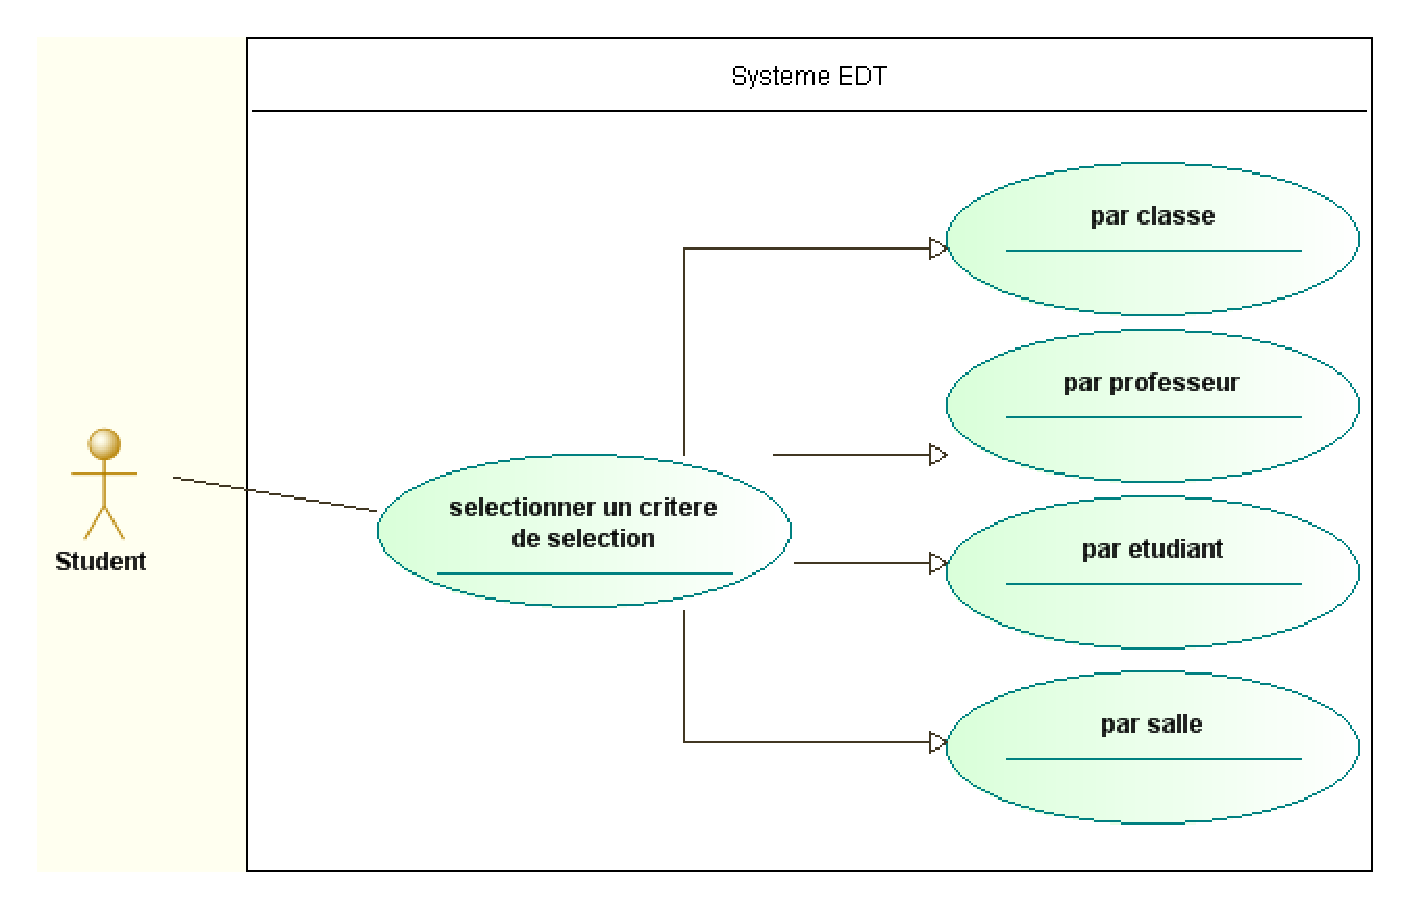
\includegraphics[width=15cm]{fig-diag-use-case-4-1-1.eps}}
        \caption{Figure Use Case 4.1.1 - Séléctionner un critère de séléction}
        \label{fig-diag-use-case-4-1-1}
        \end{figure}
	%
	\clearpage
        %
        \subsection{ Diagramme de classe}
        %
        \subsubsection{ Entités et contraintes}
        %
        \begin{itemize}
        \item \textit{Personne} :
                \begin{itemize}
                \item Une Personne possède les attributs : \textbf{Un seul} "\textbf{Nom}", \textbf{un seul} "\textbf{Prénom}", \textbf{un seul} "\textbf{Mot de passe}" et de \textbf{1..10} "\textbf{Adresse mail}".
                \end{itemize}
        \item \textit{Etudiant} :
                \begin{itemize}
                \item Un Etudiant est une Personne.
                \item Un Etudiant a \textbf{un unique} numéro "\textbf{INE}".
                \item Un Etudiant appartient à \textbf{un seul} Groupe de TD.
                \end{itemize}
        \item \textit{Professeur} :
                \begin{itemize}
                \item Un Professeur est une Personne.
                \item Un Professeur possède \textbf{un unique} numéro "\textbf{Harpège}".
                \item Un Professeur enseigne \textbf{0..*} Cours.
                \end{itemize}
        \item \textit{Administrateur} :
                \begin{itemize}
                \item Un Administrateur est une Personne.
                \item Un Administrateur possède l'attribut "\textbf{Identifiant}" avec \textbf{une seule} instance.
                \end{itemize}
        \item \textit{Groupe de TD} :
                \begin{itemize}
                \item Un Groupe de TD est composé de \textbf{1..*} Etudiant.
                \item Un Groupe de TD a un seul "\textbf{numéro de groupe}".
                \item Un Groupe de TD est en relation avec \textbf{une seule} Filière.
                \item Un Groupe de TD est en relation avec \textbf{0..*} Cours.
                \end{itemize}
        \item \textit{Filière} :
                \begin{itemize}
                \item Une Filière est en relation avec \textbf{1..*} Groupe de TD.
                \item Une Filière possède un "\textbf{Nom filière}".
                \end{itemize}
        \item \textit{Année d'étude} :
                \begin{itemize}
                \item Une Année d'étude est une classe association entre Filière et Groupe de TD.
                \item Une Année d'étude possède un "\textbf{numéro d'année}".
                \item Une Année d'étude possède un "\textbf{niveau d'étude}".
                \end{itemize}
        \item \textit{Matière} :
                \begin{itemize}
                \item Une Matière est associé à \textbf{1..*} Cours.
                \item Une Matière est composé d'\textbf{un unique} attribut "\textbf{Nom matière}".
                \end{itemize}
        \item \textit{Cours} :
                \begin{itemize}
                \item Un Cours possède un attribut "\textbf{Description du cours}".
                \item Un Cours est en relation avec \textbf{une seul} Matière.
                \item Un Cours est en relation avec \textbf{1..*} Groupe de TD.
                \item Un Cours est encadré par \textbf{un seul} Professeur.
                \item Un Cours se passe dans \textbf{une seule} Salle.
                \item Un Cours se déroule pendant \textbf{une seule} Horaire.
                \end{itemize}
        \item \textit{Salle} :
                \begin{itemize}
                \item Une Salle permet l'enseignement de \textbf{0..*} Cours.
                \item Une Salle possède les attributs : un seul "\textbf{Numéro de salle}", une "\textbf{Capacité}", et une "\textbf{Spécification}".
                \item Une Salle compose \textbf{un seul} Batiment.
                \end{itemize}
        \item \textit{Batiment} :
                \begin{itemize}
                \item Un Batiment est composé de \textbf{1..*} Salle.
                \item Un Batiment a l'attribut "\textbf{Nom batiment}".
                \item Un Batiment a l'attribut "\textbf{Adresse batiment}".
                \end{itemize}
        \item \textit{Date} :
                \begin{itemize}
                \item Une Date est en relation avec \textbf{0..*} Horaire.
                \item Une Date possède les attributs \textbf{uniques} : "\textbf{Année}", "\textbf{Mois}" et "\textbf{Jour}".
                \end{itemize}
        \item \textit{Horaire} :
                \begin{itemize}
                \item Une Horaire est en relation avec \textbf{0..*} Cours.
                \item Une Horaire est en relation avec \textbf{une seule} Date.
                \item Une Horaire possède les attributs : \textbf{une seule} "\textbf{Heure de début}" et \textbf{une seule} "\textbf{Heure de fin}".
                \end{itemize}
        \end{itemize}
	%
	\subsubsection{ Représentation UML}
	%
	\begin{figure}[h]
        \shadowbox{\large\bf\includegraphics[width=15cm]{fig-diag-class-1.eps}}
        \caption{Figure Diagramme Classe}
        \label{fig-diag-class-1}
        \end{figure}
	%
	\clearpage
        %
        %\subsection{Diagramme d'état}
        %
        \subsection{Diagramme d'activité}
        %
        \begin{figure}[h]
        \shadowbox{\large\bf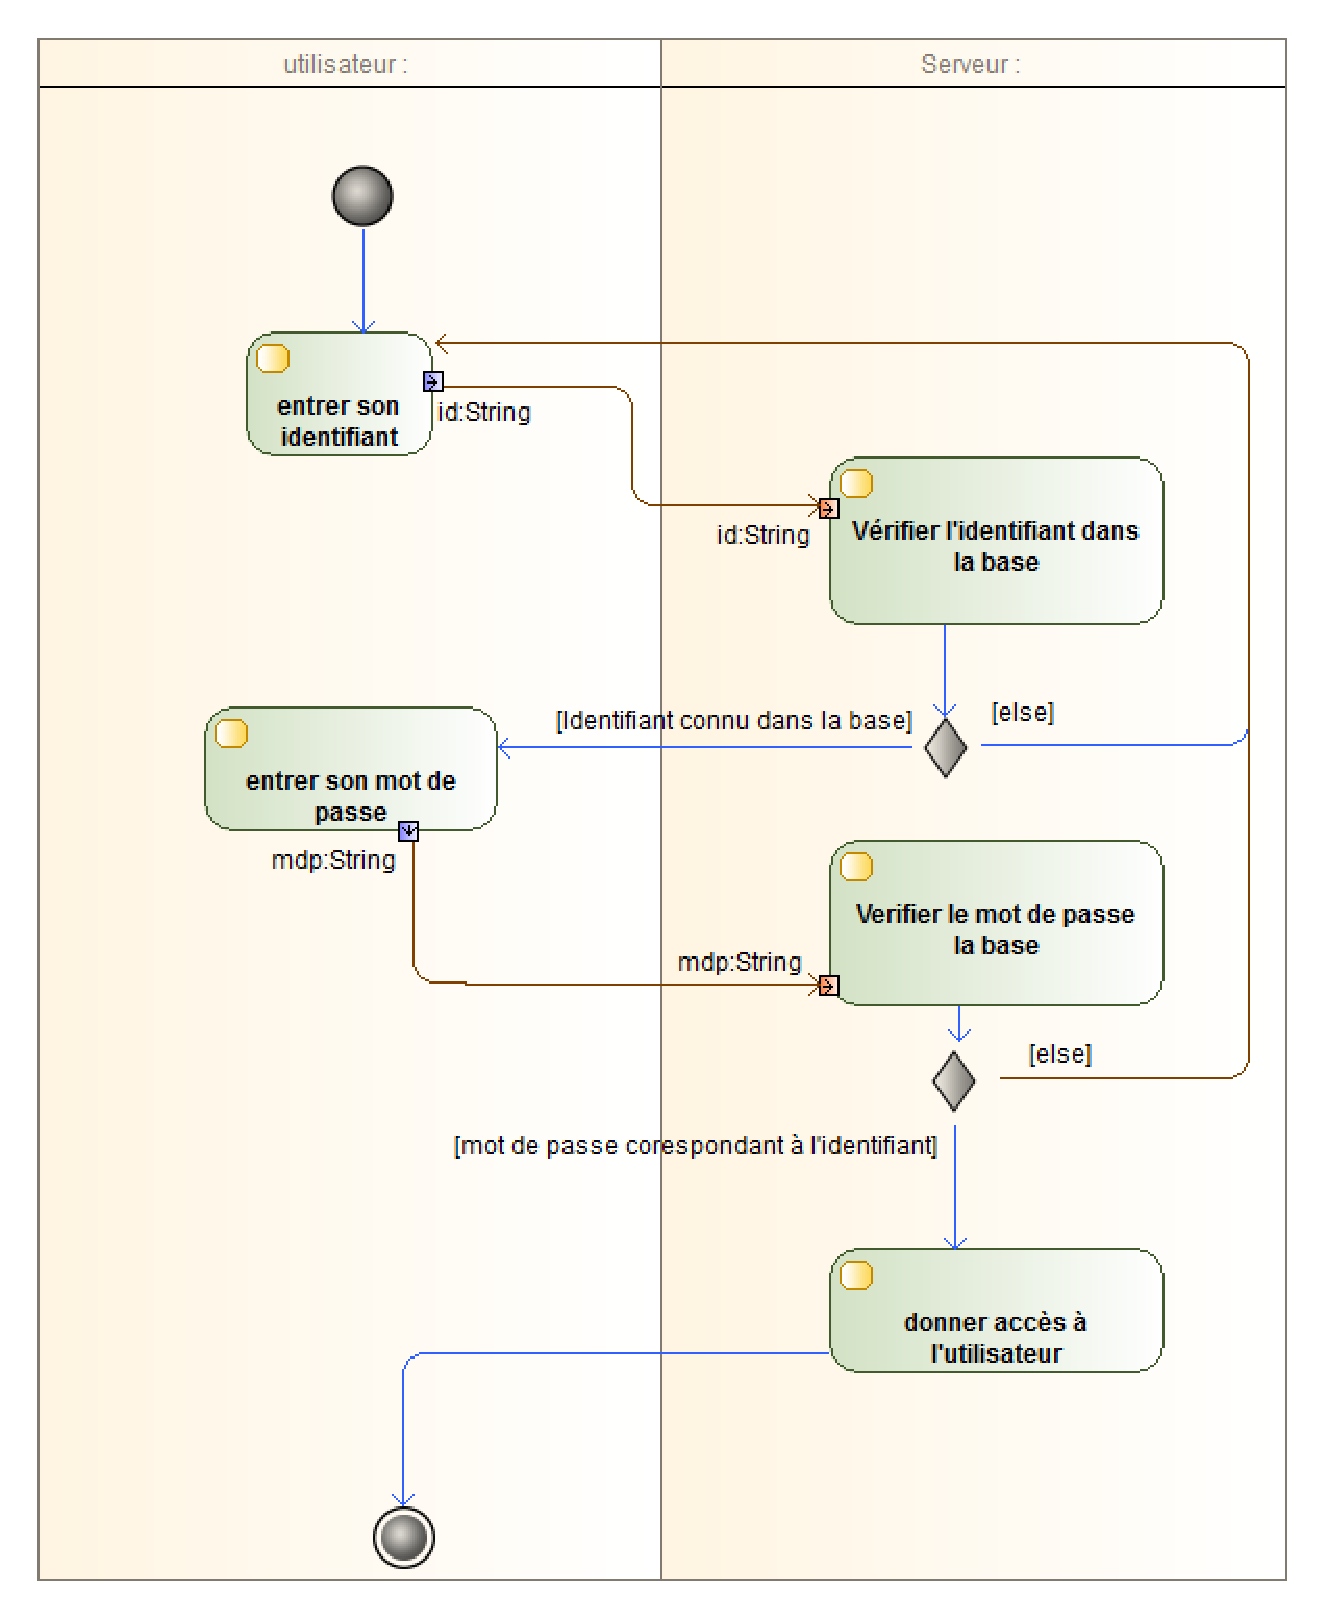
\includegraphics[width=14.5cm]{fig-diag-act-connexion.eps}}
        \caption{Figure Diagramme d'activité - Connexion}
        \label{fig-diag-activite-connexion}
        \end{figure}
        %
        Ce diagramme d'activité représente la procédure de connexion à notre système d'emploi du temps.\\
        Il faut donc bien vérifier si le nom d'utilisateur et le mot de passe correspondent entre eux et surtout si l'utilisateur est connu du système.
        %
        \clearpage
        %
        \begin{figure}[h]
        \shadowbox{\large\bf\includegraphics[width=14.5cm]{fig-diag-act-consulter.eps}}
        \caption{Figure Diagramme d'activité - Consulter un emploi du temps}
        \label{fig-diag-activite-consulter}
        \end{figure}
        %
        Ce diagramme d'activité représente la procédure pour consulter un emploi du temps.\\
        Il concerne tous les utilisateurs (Etudiant, Professeur et Administrateur).\\
        Bien entendu cette procédure n'est valable que si l'utilisateur qui consulte est passé par la procédure de connexion (voir diagramme d'activité Connexion).
        %
        \clearpage
        %
        \begin{figure}[h]
        \shadowbox{\large\bf\includegraphics[width=14cm]{fig-diag-act-modifier-administrateur-part1.eps}}
        \caption{Figure Diagramme d'activité - Modifier administrateur partie 1}
        \label{fig-diag-activite-modifier-admin-part1}
        \end{figure}
        %
        La deuxième partie de ce diagramme ce trouve sur la page suivante (voir Digramme d'activité Modifier administrateur partie 2).
        %
        \clearpage
        %
        \begin{figure}[h]
        \shadowbox{\large\bf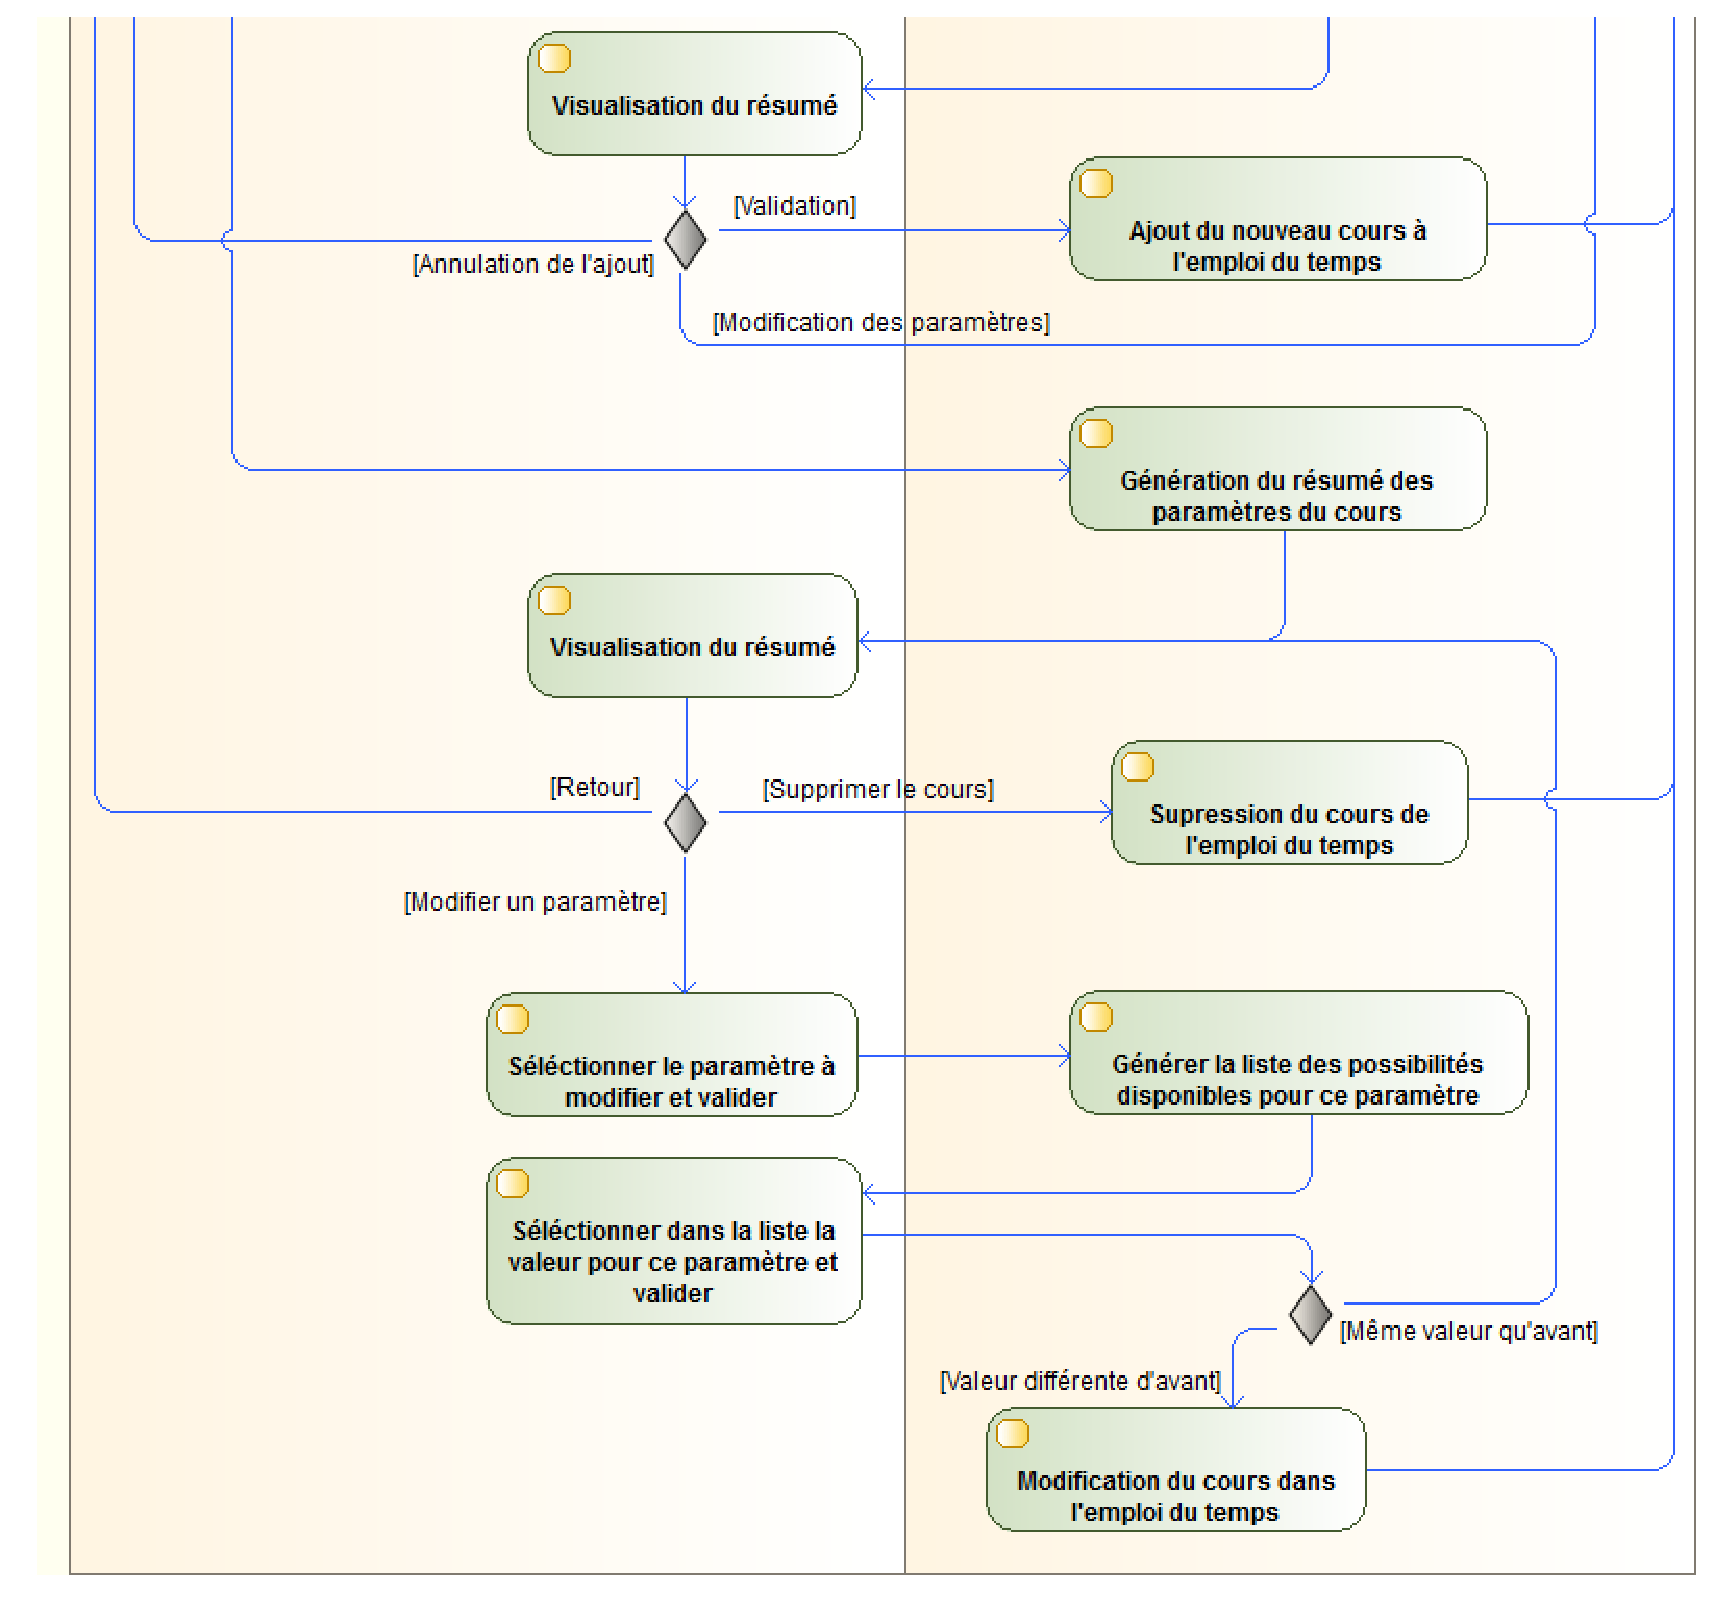
\includegraphics[width=14cm]{fig-diag-act-modifier-administrateur-part2.eps}}
        \caption{Figure Diagramme d'activité - Modifier administrateur partie 2}
        \label{fig-diag-activite-modifier-admin-part2}
        \end{figure}
        %
        Ce diagramme d'activité représente la procédure pour modifier un emploi du temps lorsqu'on est un Administrateur.\\
        Bien entendu cette procédure n'est valable que si l'Administrateur s'est connecté à l'aide de la procédure de connexion (voir diagramme d'activité Connexion).\\
        La première partie de ce diagramme ce trouve sur la page précédente (voir Diagramme d'activité Modifier administrateur partie 1).
        %
	\clearpage
        %
        %\subsection{Diagramme de séquence}
        %
        \subsection{ Liste des fonctionnalités du produit}
	%
        Les fonctionnalités sont :
	\begin{itemize}
		\item Se connecter
		\begin{itemize}
			\item Entrée : Nom d'utilisateur et mot de passe
			\item Sortie : Page d'erreur de connexion ou page d'accueil
			\item Dépendances : Aucune
		\end{itemize}
		%\item Gérer son espace utilisateur
		%\begin{itemize}
			%\item Entrée : Aucune
			%\item Sortie : Page d'erreur si non connecté ou page de modification
			%\item Dépendances : Être connecté
		%\end{itemize}
		\item Consulter un emploi du temps
		\begin{itemize}
			\item Entrée : Emploi du temps choisi
			\item Sortie : Page d'erreur si non connecté ou page de l'emploi du temps
			\item Dépendances : Être connecté
		\end{itemize}
		\item Modifier un emploi du temps
		\begin{itemize}
			\item Entrée : Emploi du temps choisi
			\item Sortie : Page d'erreur si non connecté ou page de l'emploi du temps modifiable
			\item Dépendances : Être connecté en temps qu'administrateur d'emploi du temps
		\end{itemize}
		\item Gérer les utilisateur
		\begin{itemize}
			\item Entrée : Utilisateur choisi
			\item Sortie : Page d'erreur si non connecté ou page d'utilisateur
			\item Dépendances : Être connecté en temps qu'administrateur d'emploi du temps
		\end{itemize}
		\item Changer ses informations
		\begin{itemize}
			\item Entrée : Aucune
			\item Sortie : Page d'erreur si non connecté ou page d'information modifiable
			\item Dépendances : Être connecté
		\end{itemize}
		\item Chercher un emploi du temps
		\begin{itemize}
			\item Entrée : Critères de recherche
			\item Sortie : Page d'erreur si non connecté ou page de resultat
			\item Dépendances : Être connecté
		\end{itemize}
		\item Modifier un cours
		\begin{itemize}
			\item Entrée : Cours choisi
			\item Sortie : Page d'erreur si non connecté ou page du cours modifiable
			\item Dépendances : Être connecté et soit être administrateur ou l'auteur du cours choisi
		\end{itemize}
		%\item Chercher un emploi du temps
		%\begin{itemize}
			%\item Entrée : Critères de recherche
			%\item Sortie : Page d'erreur si non connecté ou page de resultat
			%\item Dépendances : Être connecté
		%\end{itemize}
	\end{itemize}
        %
        \section{ Autres exigences}
        %
        \subsection{Exigences de performance}
        %
        Le site doit répondre vite aux demandes, donc nos requêtes doivent être rapide à traiter.
        %
        \subsection{ Exigences logique de la base de données}
        %
        Peu de redondance, voir pas du tout dans la base de donnée afin de rester propre au niveau de la mémoire utilisé.
        %
        \subsection{Spécifications du logiciel}
        %
        Programmé en PHP et rendu fait en HTML et CSS.
        %
        \subsection{Fiabilités}
        %
        Il faut que le logiciel soit disponible durant la journée, cependant s'il ne l'est pas la nuit, ce n'est pas grave, du moment qu'il soit rétabli rapidement le matin. 
        %
        \subsection{Disponibilités}
        Le système est présent principalement sur un site internet, permettant une compatibilité avec tous les navigateurs.
        %
        \subsection{ Sécurité}
        %
        L'accès à la plateforme du système présenté, se fait à l'aide d'identifiants (voir contrainte utilisateur un peu après), et non autrement afin de garder une sécurité du système. Bien faire attention afin que seul les administrateur puissent modifier les différents emplois du temps, et qu'un cours est modifiable uniquement par l'administrateur ou le professeur qui le fait. 
        %
        \subsection{Maintenance}
        %
        Les maintenance doivent être fait uniquement la nuit, afin de ne pas bloquer les étudiants et les professeurs la journée lors des cours.
        %
        \subsection{ Portabilité}
        %
        Le système est prévu pour une plateforme en ligne sur internet, ainsi le système sera accessible sur tous les systèmes d'exploitation du moment qu'ils possèdent un navigateur. Les capacité demandé devrons cependant être minimale pour permettre un accès rapide (chargement des pages sur internet rapide), pour de petite connexion ou des navigateurs un peu ancien.
        %
        %\subsection{ Autres exigences}
        %
        %\clearpage
	%
	\clearpage
        %
\end{document}
